\part{Part 4: Applications}

\graphicspath{ {./Pictures/} }
\chapterimage{chapter_head_2.pdf} % Chapter heading image

%++++++++++++++++++++++++++++++++++++++++++++++++++++++++++++++
\chapter{Introduction}
%++++++++++++++++++++++++++++++++++++++++++++++++++++++++++++++
\section{Gmsh}
%++++++++++++++++++++++++++++++++++++++++++++++++++++++++++++++
Gmsh is an 2D/3D finite element mesh generator included in built-in CAD engine and post-processor. Gmsh is developed in order to provide a fast, light and user-friendly meshing environment and visualization capabilities. This software is open source and the source code of Gmsh for various operating platforms (i.e. Windows, Mac and Unix) can be downloaded from http://gmsh.info. Gmsh contains four modules for geometry definition, meshing, solving and post-processing. each module has its own specifications as input and it can be controlled and manipulated interactively using the graphical user-interface (GUI), Gmsh's own scripting language (.geo file) or even using the C++, C or Python Application Programming Interface (API).
Once we execute Gmsh, the module panel appears normally in left-hand side of window, including:
\begin{itemize}
    \item \textbf{Geometry}
    \item \textbf{Mesh}
    \item \textbf{Solver}
\end{itemize}
Now, we try to explain each module separately and explain important features for each of them. The \textbf{Geometry} is a module that you can design your own geometry or import CAD design. A geometry is Gmsh is defined using its Boundary representation. It means a volume is made up of different surfaces, and each surface is made up of different curvatures or lines. Then, each curvature or line is bounded by two end points. Therefore, this representation shows the way we should take to design a 2D/3D geometry.
Therefore, to define a shape in space, set of points are specified and the connections between these pints are built by straight lines or curvatures. Now, Gmsh can figure out surfaces based on the boundaries defined (line/curvature/end point). Later, based on the surfaces defined, Gmsh ca generates volume of geometry in space.

This module has some sections that help you to define geometric parameters and shape of your design. Some of important sections of this module is enlisted and described as follows:
\begin{itemize}
    \item \textbf{Elementary entities}: helps to add, merge, split or delete points, lines, curves, faces or volumes we defined.
    \item \textbf{Physical groups}: manages boundary conditions and physical properties (i.e. fluid or solid) of predefined geometry.
    \item \textbf{Reload script}: reads and load the data defined predefined geometry from Gmsh's own language script saved in .geo file.
    \item \textbf{Edit script}: allows you to edit the .geo file manually to change any specifications.
\end{itemize}
It is worth pointing out that all specifications of geometry are saved in .geo file, this helps operator to manually manipulate geometry or any other specifications. 
After building geometry and defining boundary conditions via \textbf{Geometry} module, the next step is to make finite element mesh of the geometry model using \textbf{Mesh} module. This module helps to define our geometry model by simple geometrical elements, such as: lines, triangles, tetrahedra, hexahedra and pyramids. Gmsh uses different algorithms for generating mesh automatically and the type of mesh in Gmsh is unstructured by default, otherwise we specify to generate structured one. \textbf{Mesh} module has also some sections that help to specify the type, number and density of mesh in domain. Here, some of important sections are provided as follows:
\begin{itemize}
    \item \textbf{Define}: sets number of grids as well as growth ratio on the boundaries. Additionally, it specifies the mesh type (whether Structured or Unstructured).
    \item \textbf{2D/3D}: makes mesh for surfaces/volumes existed in domain. It automatically generate mesh based on the specifications provided in \textbf{Define} section.
    \item \textbf{Set order 1, 2, or 3}: Since the grid points in the mesh are connected to each other by straight lines (\textbf{Set order 1}), sometimes it is inefficient to define a geometry's curvatures using these straight lines. However, to overcome this problem, the mesh lines that define these curvatures can be more flexible and defined as polynomial (\textbf{Set order 2 or 3}). This feature helps to have more smooth mesh just beside curvatures to increase mesh quality in these regions.
    \item 
\end{itemize}
Additionally, there is another module named \textbf{Solver}, which embed Gmsh directly to another solver.
In this section, we are trying to explain how to use Gmesh in order to design and build a mesh-file for CFD application. This module makes an interface to share parameters and modeling information with different solvers. ONLAB (http://onelab.info) is one of examples that is used for this purpose. Explaining more details about this module is beyond the scope of this book.
%++++++++++++++++++++++++++++++++++++++++++++++++++++++++++++++
\section{SU2}
%++++++++++++++++++++++++++++++++++++++++++++++++++++++++++++++
\section{Paraview}
%++++++++++++++++++++++++++++++++++++++++++++++++++++++++++++++
\chapter{Inviscid NACA 0012}
%++++++++++++++++++++++++++++++++++++++++++++++++++++++++++++++
\section{Problem Description}
In this tutorial, we are going to explain how to simulate inviscid flow around an NACA0012 airfoil. Since the flow is assumed to be inviscid, we apply Euler equation for flow modeling. Please note that at high Reynolds numbers, the flow could be assumed to be inviscid, since viscosity term in Navier-Stokes equations becomes negligible. For this example, the flow specifications are provided as follows:
\begin{itemize}
    \item Pressure = 101,325 Pa
    \item Temperature = 273 K
    \item Mach number = 0.8
    \item Angle of attack = 1.25 degree
\end{itemize}
The tutorial has two parts: Flow Solution and Post-Processing. In the first part, we explain how to manage prerequisite files and settings, and how to run the CFD simulation using SU2. In the second part, we explain how to use Paraview software to visualize data obtained form SU2.
%++++++++++++++++++++++++++++++++++++++++++++++++++++++++++++++
\section{Flow solution}
To run the simulation, the SU2 needs two essential files: configuration file (.cfg) and mesh file (.su2). In this example, the following files are located in \textit{01Quickstart} folder:
\begin{enumerate}
\item \textit{inv\_NACA0012}.cfg as a configuration file.
\item \textit{mesh\_NACA0012\_inv}.su2 as a mesh file.
\end{enumerate}
The next step is to copy these two files in directory of SU2, where the execution and script files are located there. To run this simulation, open the command line terminal and enter the following commands:
\begin{table}[htbp]
    \centering
    \begin{tabular}{|l|l|}
    \hline
    Windows     & \begin{tabular}{c} \$ cd "where you saved the package" \\ \$ SU2\_CFD.exe inv\_NACA0012.cfg \end{tabular}
    \\
    \hline
    OSX     & \begin{tabular}{c} \$ cd "where you saved the package" \\ \$ SU2\_CFD.exe inv\_NACA0012.cfg \end{tabular}
    \\
    \hline
    \end{tabular}
\end{table}

The SU2 solver will commence calculation and print out the residuals at every iteration until the specified convergence criteria is achieved. After calculations are done, the following output files should be generated and saved in the SU2 folder:
\begin{itemize}
    \item \textit{flow}.vtk: contains the full volume flow solution.
    \item \textit{force\_breakdown}.dat: contains forces and moment on the airfoil.
    \item \textit{history}.vtk: contains convergence history of calculations.
    \item \textit{restart\_flow}.dat: for restarting simulation.
    \item \textit{surface\_flow}.vtk: flow solution on the surface of the airfoil.
    \item \textit{surface\_flow}.csv: comma separated values of flow solution on the airfoil (If you want to plot data in another software, like Microsoft Excel, you can use this file).
\end{itemize}
Please keep in mind that every time you run SU2, the output data will be overwritten. Hence, before launching new simulation, you could make a new folder and transfer your data from previous simulation to this folder.
%++++++++++++++++++++++++++++++++++++++++++++++++++++++++++++++
\section{Post-processing}
In this section, we explain how to use Paraview to visualize CFD data for this example. First of all, install Paraview (this tutorial uses Paraview 3.12.0) if you do not have it on your computer. Otherwise, take following steps for visualization:
%--------------------------------------------------------------
\subsection{Load Solution File:}
Launch Paraview. Go to \textbf{File} $\rightarrow$ \textbf{Open}, and then select \textit{flow}.vtk file. On the left-hand side of Paraview window you will see the file appears under \textbf{builtin} in \textbf{Pipeline Browser}. Now press \textbf{Apply} button in \textbf{Properties} tab, just right under the  \textbf{Pipeline Browser}. After taking these steps, your file is loaded by software and is ready to visualize (Fig.\ref{fig:load}).
\begin{figure}[htbp]
    \centering
    \includegraphics[width=0.4\textwidth]{tut01/loadvtkfile.pdf}
    \caption{Loading .vtk file in the \textbf{Pipeline Browser}.}
    \label{fig:load}
\end{figure}
%--------------------------------------------------------------
\subsection{Visualize Mesh Domain}
In order to view mesh, according to Fig.\ref{fig:wireframe}, select \textit{Solid Color} with \textit{Wireframe} in the toolbar. Then, you can zoom in to see mesh around the airfoil like Fig.\ref{fig:mesh}. As you can see, the mesh around the NACA0012 is unstructured, and the grids are clustered around the leading and trailing edges of the airfoil.
\begin{figure}[htbp]
    \centering
    \includegraphics[width=0.6\textwidth]{tut01/wireframe.pdf}
    \caption{How to display mesh in computational domain.}
    \label{fig:wireframe}
\end{figure}
\begin{figure}[htbp]
    \centering
    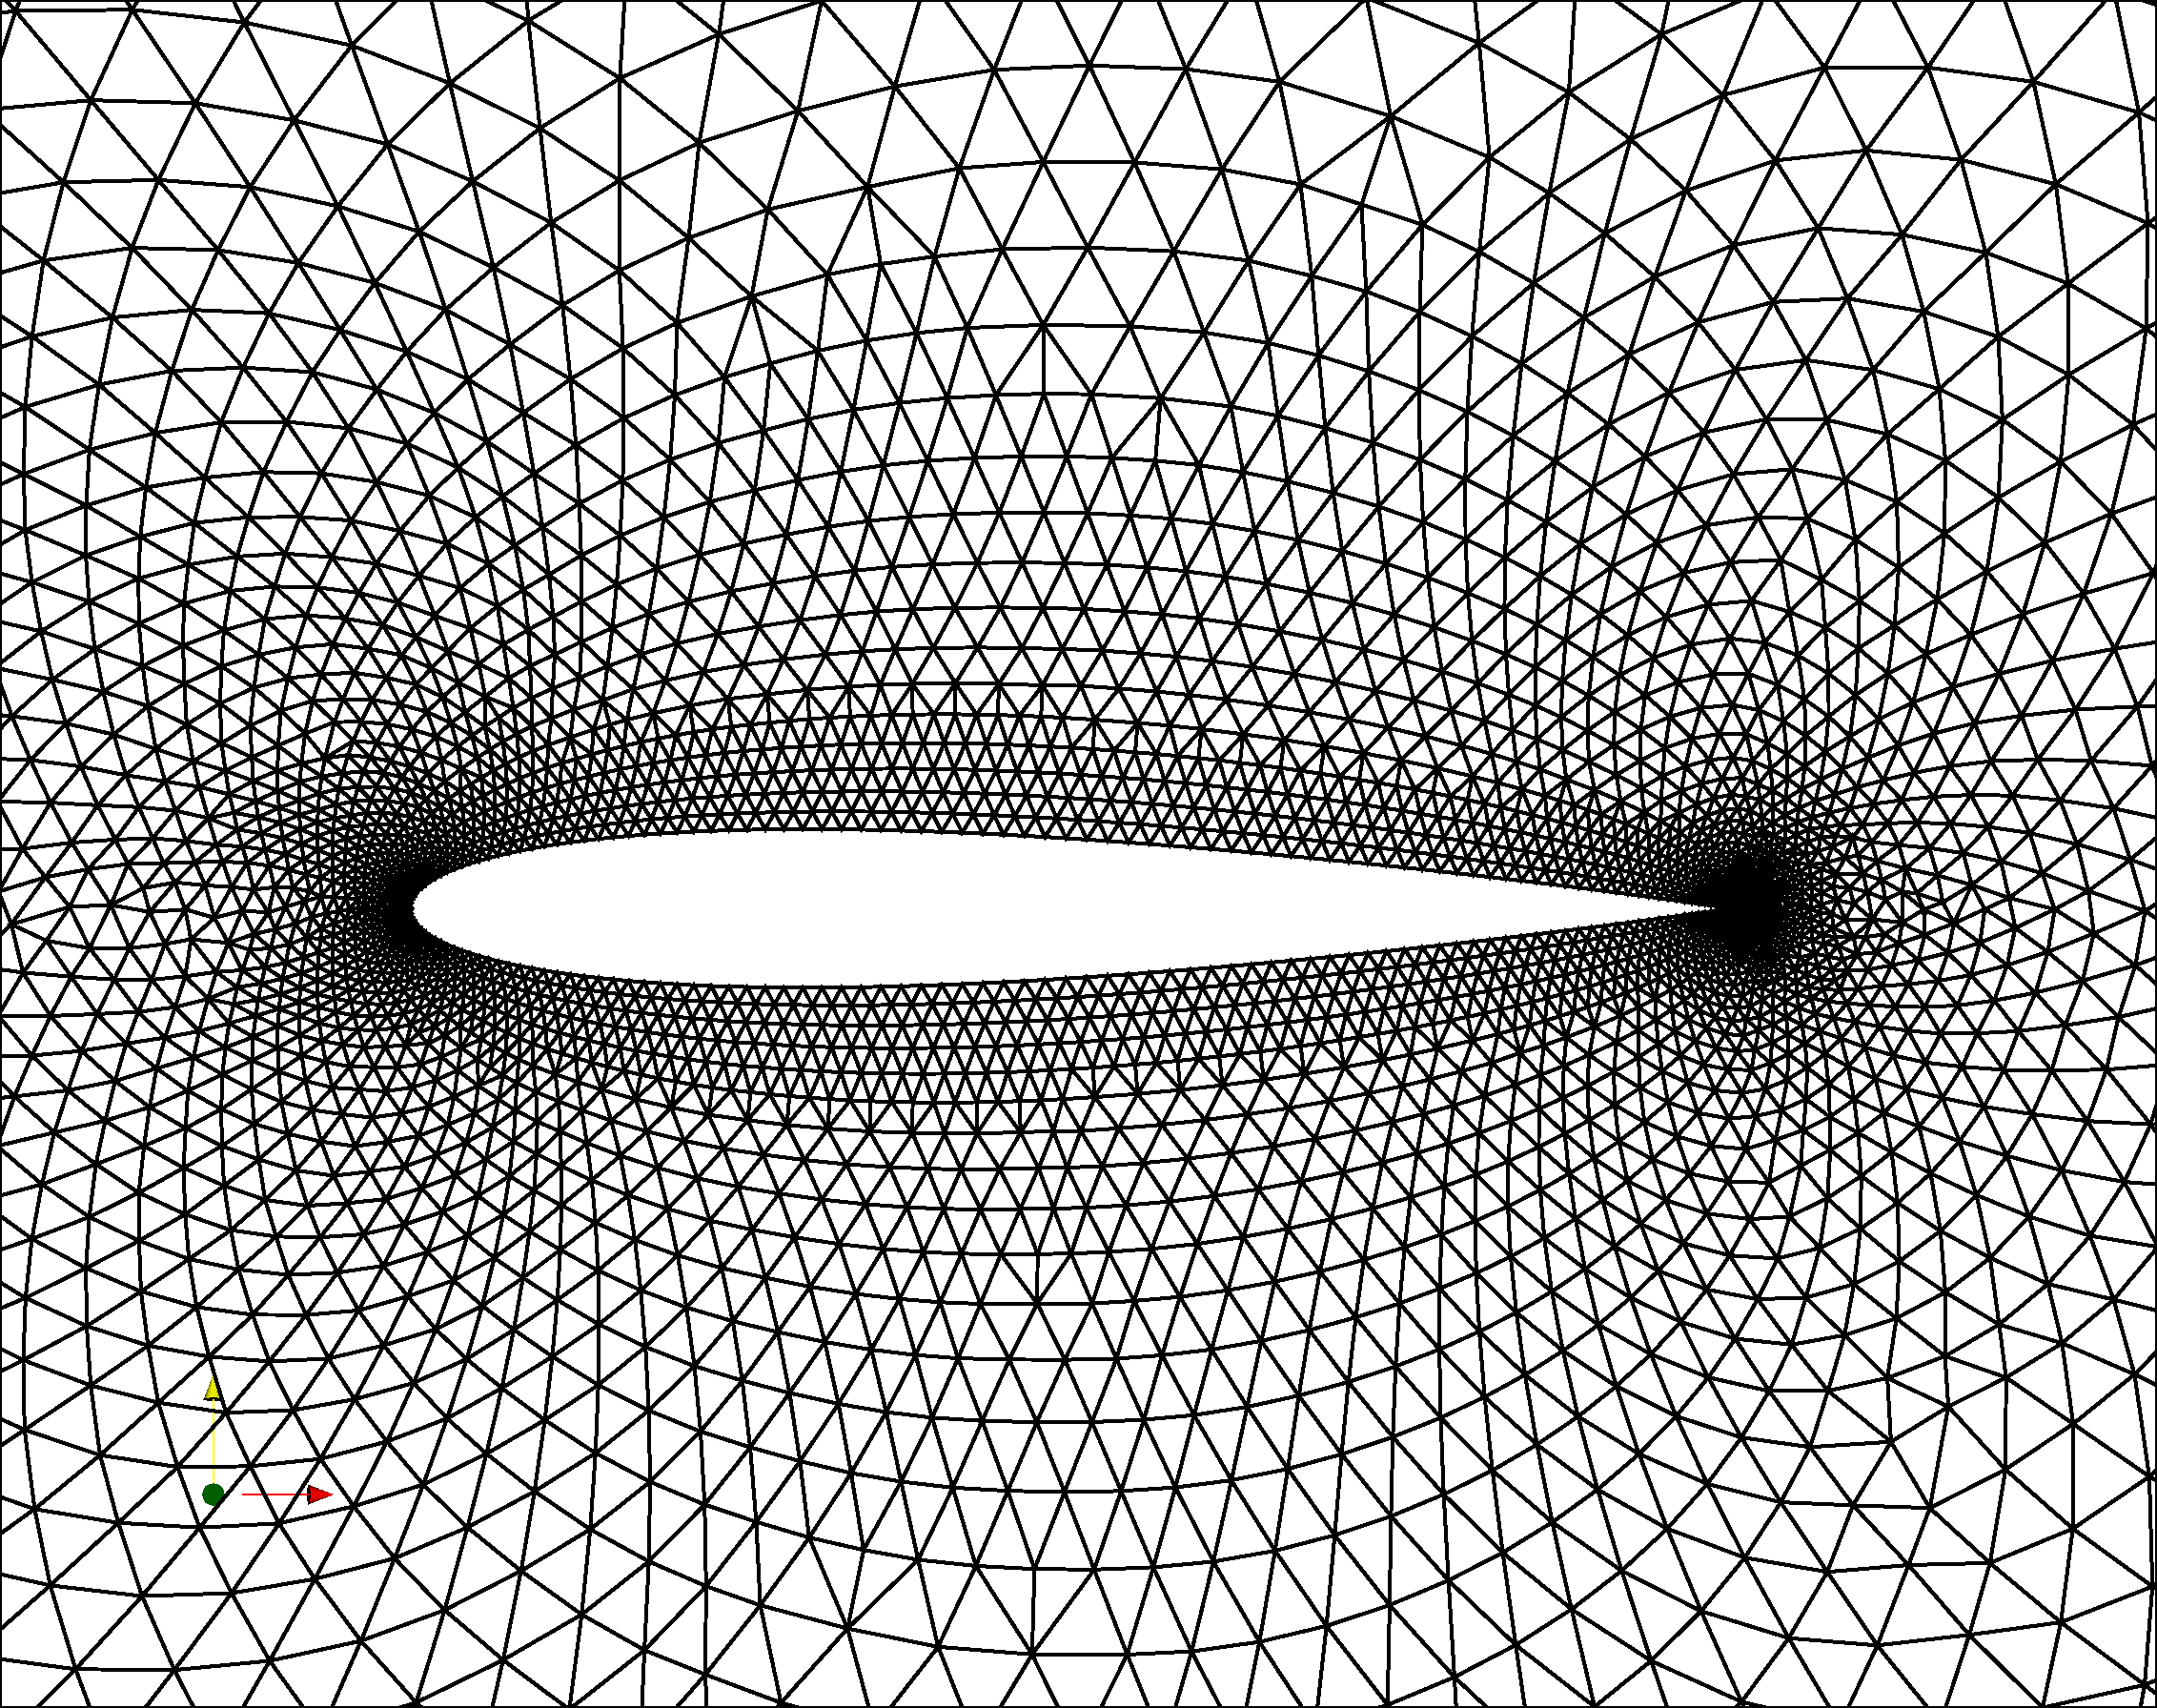
\includegraphics[width=.75\textwidth]{tut01/mesh.pdf}
    \caption{Unstructured mesh around NACA0012.}
    \label{fig:mesh}
\end{figure}
%--------------------------------------------------------------
\subsection{Visualize Pressure Contour}
In order to visualize pressure contour, click on the \textit{flow}.vtk from \textbf{Pipeline Browser} to activate the file, and then click on the \textbf{Properties} tab. According to Fig.\ref{fig:colorby}, in \textbf{Coloring} section, select \textit{Pressure} from drop-down menu. To change color settings for the pressure, you can also click on the \textbf{Edit} under the \textbf{Coloring}. Normally another display window appears on the right-hand side of the monitor, similar to Fig.\ref{fig:change_color_range}. Now you can change the maximum/minimum range of pressure to your desirable values by \textbf{Set Range}, or change contour colors by \textbf{Choose Preset} (Fig.\ref{fig:change_color_range}).
\begin{figure}[htbp]
    \centering
    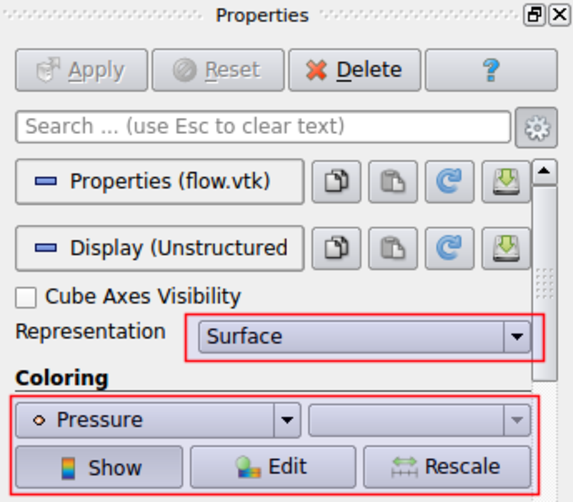
\includegraphics[width=0.4\textwidth]{tut01/contourdisplay.pdf}
    \caption{Contour settings in \textbf{Display} tab.}
    \label{fig:colorby}
\end{figure}
\begin{figure}[htbp]
    \centering
    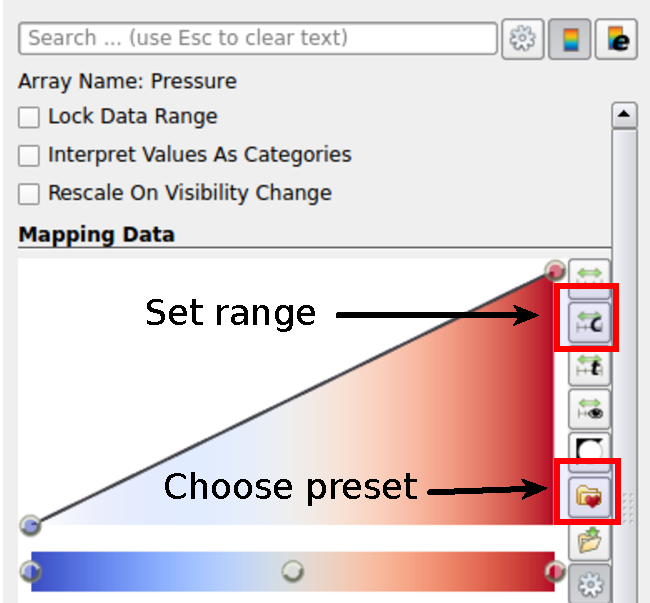
\includegraphics[width=0.5\textwidth]{tut01/colormap.pdf}
    \caption{How to change color and max/min values for contour.}
    \label{fig:change_color_range}
\end{figure}
After taking these steps, the pressure contour in the display window should be similar to Fig.\ref{fig:pressure_contour}.
\begin{figure}[htbp]
    \centering
    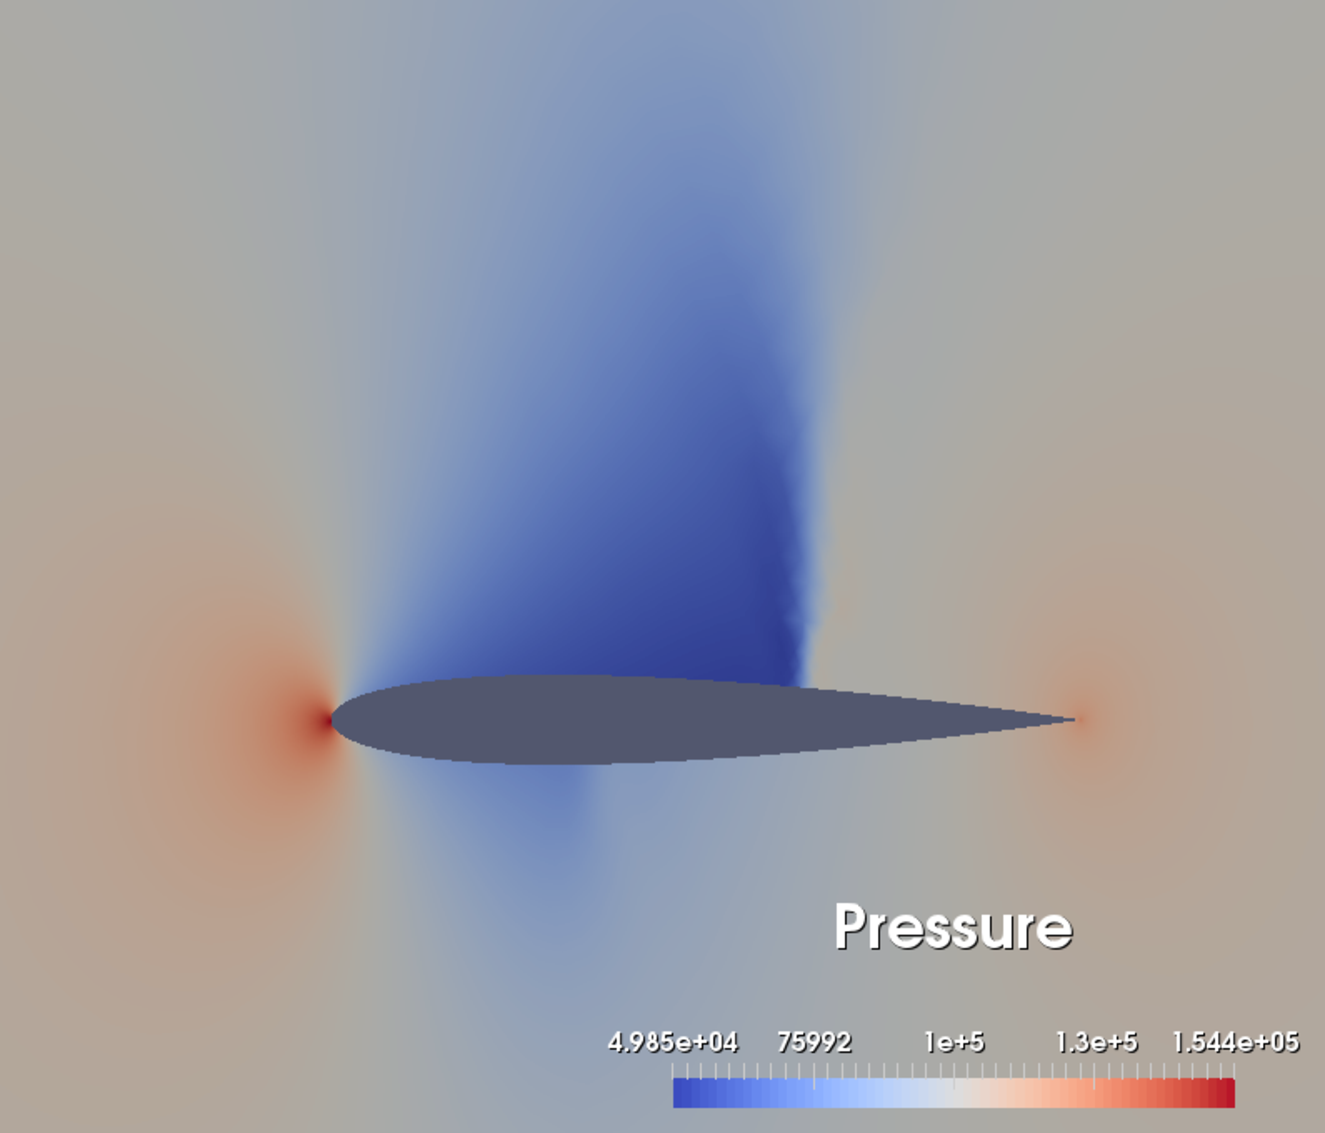
\includegraphics[width=.75\textwidth]{tut01/pressurecontour1.pdf}
    \caption{Pressure contour for NACA0012 airfoil.}
    \label{fig:pressure_contour}
\end{figure}

To add contour lines, click again on the \textit{flow}.vtk file in the \textbf{Pipeline Browser}, and then click on the \textbf{Contour} icon (Fig.\ref{fig:contour_icon}) in toolbar.
\begin{figure}[htbp]
    \centering
    \includegraphics[width=0.6\textwidth]{tut01/contourlineicon.pdf}
    \caption{Contour icon in toolbar.}
    \label{fig:contour_icon}
\end{figure}
Now you should see \textit{Contour1} appears under \textit{flow}.vtk file in the \textbf{Pipeline Browser} (Fig.\ref{fig:contour1}).
\begin{figure}[htbp]
    \centering
    \includegraphics[width=0.5\textwidth]{tut01/contour1.pdf}
    \caption{Adding \textit{Contour1} in \textbf{Pipeline Browser}.}
    \label{fig:contour1}
\end{figure}
According to Fig.\ref{fig:contourby a}, go to the \textbf{Properties} tab, and select \textit{Pressure} from \textbf{Contour By} drop-down menu. Next, click on the \textbf{New Range} icon to customize the range of pressure contour. For now, set the number of step to 20, similar to Fig.\ref{fig:contourby b}. It means the pressure contour range is equally divided by 20 portions, and the pressure values in each portion are limited by two lines in the display window. At the end, click on \textbf{Apply} to see contour lines in display window.
\begin{figure}[htbp]
    \centering
     \begin{subfigure}[b]{.4\textwidth}
         \centering
         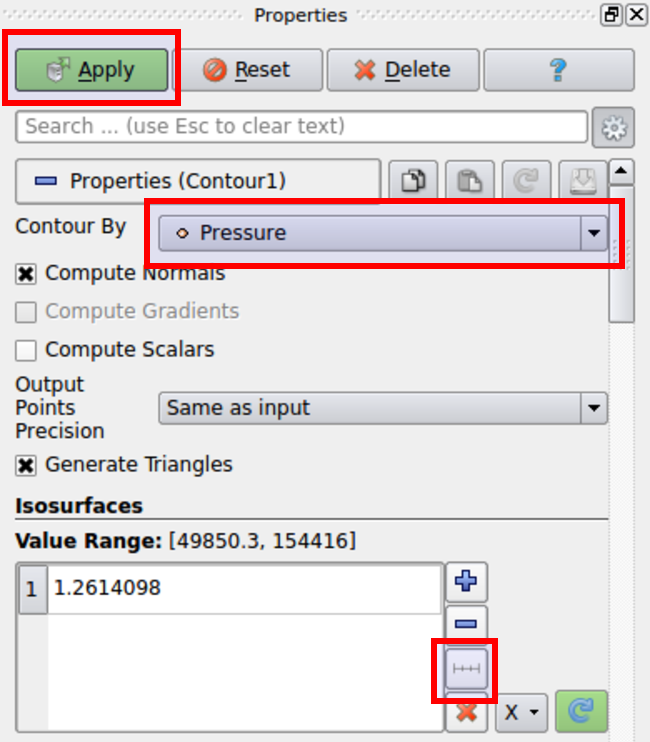
\includegraphics[width=1.0\textwidth]{tut01/contourlinenewrange.pdf}
         \caption{Define new range}
         \label{fig:contourby a}
     \end{subfigure}
     \hfill
     \begin{subfigure}[b]{.4\textwidth}
         \centering
         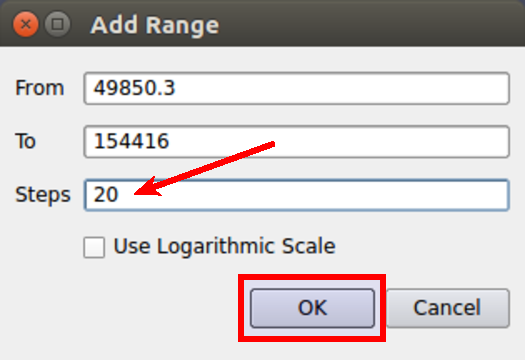
\includegraphics[width=1.0\textwidth]{tut01/addrangepdf.pdf}
         \caption{Add range}
         \label{fig:contourby b}
     \end{subfigure}     
    \caption{How to define a new range for the contour lines.}
    \label{fig:contourby}
\end{figure}
Next, as it is shown in Fig.\ref{fig:colorby2}, click on the \textbf{Display} under \textbf{Properties} tab. In \textbf{Coloring} section, select \textbf{Solid Color} form drop-down menu, and choose white color form \textbf{Edit}.
\begin{figure}[htbp]
    \centering
    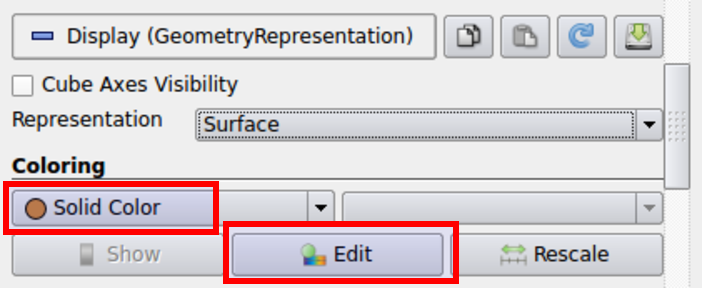
\includegraphics[width=0.6\textwidth]{tut01/coloring.pdf}
    \caption{Changing contour lines color in \textbf{Coloring} section.}
    \label{fig:colorby2}
\end{figure}
Eventually, the pressure contour with contour lines should be similar to Fig.\ref{fig:pressure_contour_lines}.
\begin{figure}[htbp]
    \centering
    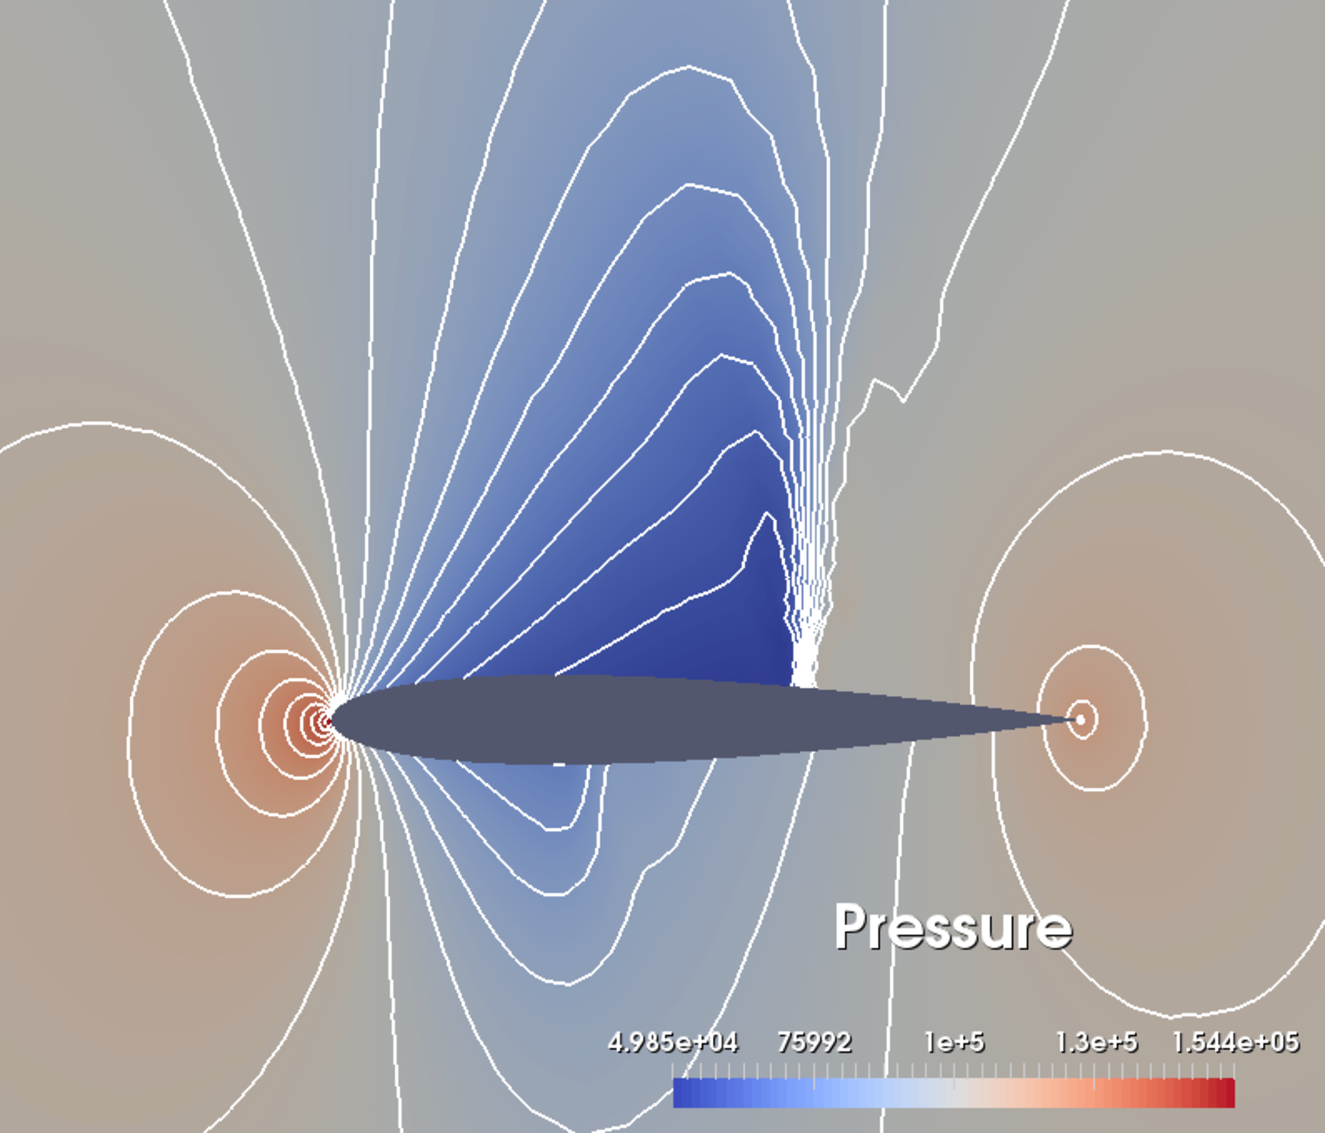
\includegraphics[width=.75\textwidth]{tut01/pressurecontour2.pdf}
    \caption{Pressure contour superimposed by contour lines around NACA0012.}
    \label{fig:pressure_contour_lines}
\end{figure}
%--------------------------------------------------------------
\subsection{Visualize Pressure Coefficient}
The pressure data on the surface of the airfoil is stored in \textit{surface\_flow}.vtk. Now the attempt is to plot it with respect to the chord line position. Therefore, go to \textbf{Open} $\rightarrow$ \textbf{File}, and select \textit{surface\_flow}.vtk. As it is shown in Fig.\ref{fig:builtin}, this file is now loaded and added to the list of items under \textbf{builtin} in \textbf{Pipeline Browser}.
\begin{figure}[htbp]
    \centering
    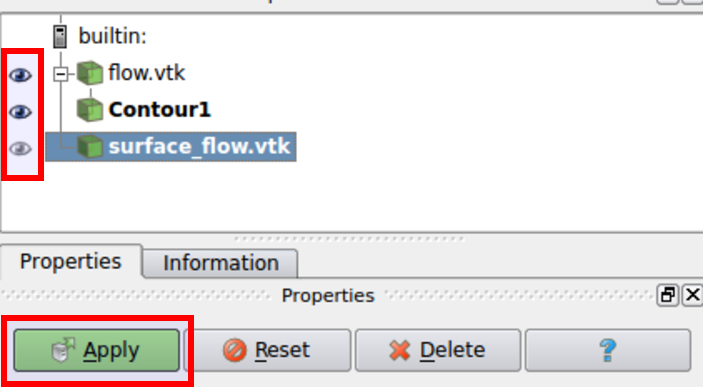
\includegraphics[width=0.5\textwidth]{tut01/eyeiconsurfaceflow.pdf}
    \caption{Loading another .vtk file in Paraview.}
    \label{fig:builtin}
\end{figure}
Note that there is an eye icon on the left-hand side of each item in \textbf{Pipeline Browser}, which enables to hide/unhide the figures being related to each item. Since we want to see pressure coefficient plot, we hide the contours by clicking on the eye icon beside \textit{flow}.vtk and \textit{Contour1}. 

According to Fig.\ref{fig:plotdata}, select \textit{surface\_flow}.vtk in \textbf{Pipeline Browser}, and then go to \textbf{Filters} $\rightarrow$ \textbf{Search} (Fig.\ref{fig:plotdata a}), and then search for \textbf{Plot Data} (Fig.\ref{fig:plotdata b}). 
\begin{figure}[htbp]
    \centering
     \begin{subfigure}[b]{.4\textwidth}
         \centering
         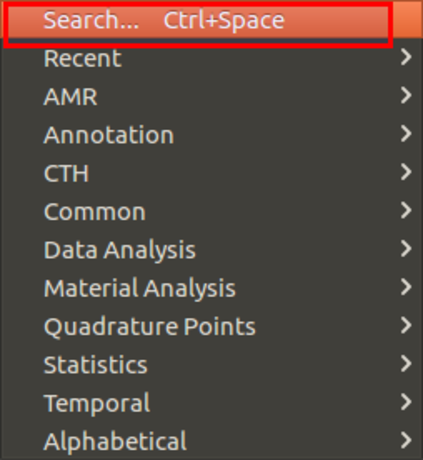
\includegraphics[width=1.0\textwidth]{tut01/filtersearch.pdf}
         \caption{Search item in \textbf{Filter}}
         \label{fig:plotdata a}
     \end{subfigure}
     \hfill
     \begin{subfigure}[b]{.4\textwidth}
         \centering
         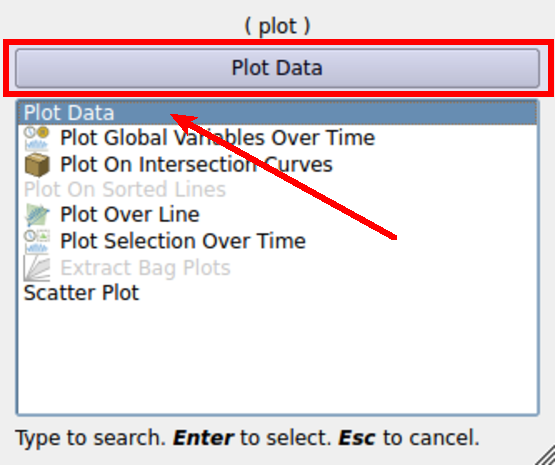
\includegraphics[width=1.0\textwidth]{tut01/plotdatasearch.pdf}
         \caption{Searching for \textbf{PotData}}
         \label{fig:plotdata b}
     \end{subfigure}     
    \caption{How to plot data.}
    \label{fig:plotdata}
\end{figure}

After taking this step, as it is shown in Fig.\ref{fig:plotdata-list}, \textit{PlotData1} item is added to the list in the \textbf{Pipeline Browser}. Then, hide (deactivate) all items in the list of \textbf{Pipeline Browser} except \textit{PlotData1} by clicking on the eye icons beside each item, and later, click on \textbf{Apply} for the next step.
\begin{figure}[htbp]
    \centering
    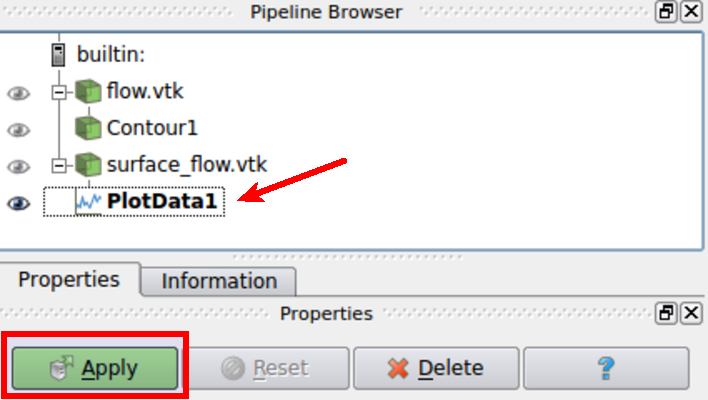
\includegraphics[width=0.5\textwidth]{tut01/plotdata1.pdf}
    \caption{Adding \textit{PlotData1} to \textbf{Pipeline Browser}.}
    \label{fig:plotdata-list}
\end{figure}
According to Fig.\ref{fig:pointsx}, from \textbf{Display} in \textbf{Properties} tab, deactivate \textbf{Use Index For XAxis}, and then select \textit{Points\_X} from drop-down menu. 
\begin{figure}[htbp]
    \centering
    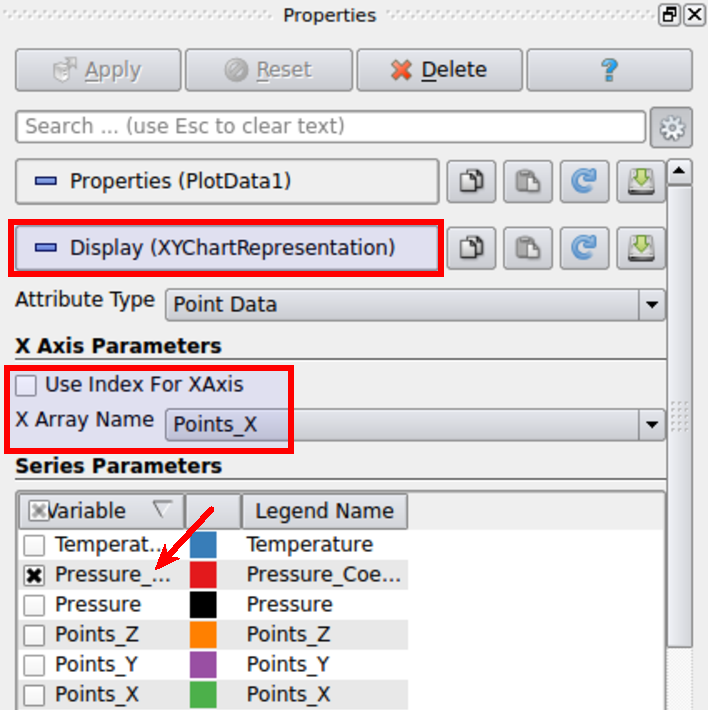
\includegraphics[width=0.5\textwidth]{tut01/plotcurvesetting.pdf}
    \caption{Plot settings for pressure coefficient along the chord line.}
    \label{fig:pointsx}
\end{figure}
In the \textbf{Series Parameters} in the same tab, unclick all variables except for \textit{Pressure\_Coefficient}. This allows you to have only one plot for pressure coefficient versus chord line. The pressure plot in the display window should be similar to Fig.\ref{fig:surface_pressure}.
\begin{figure}[htbp]
    \centering
    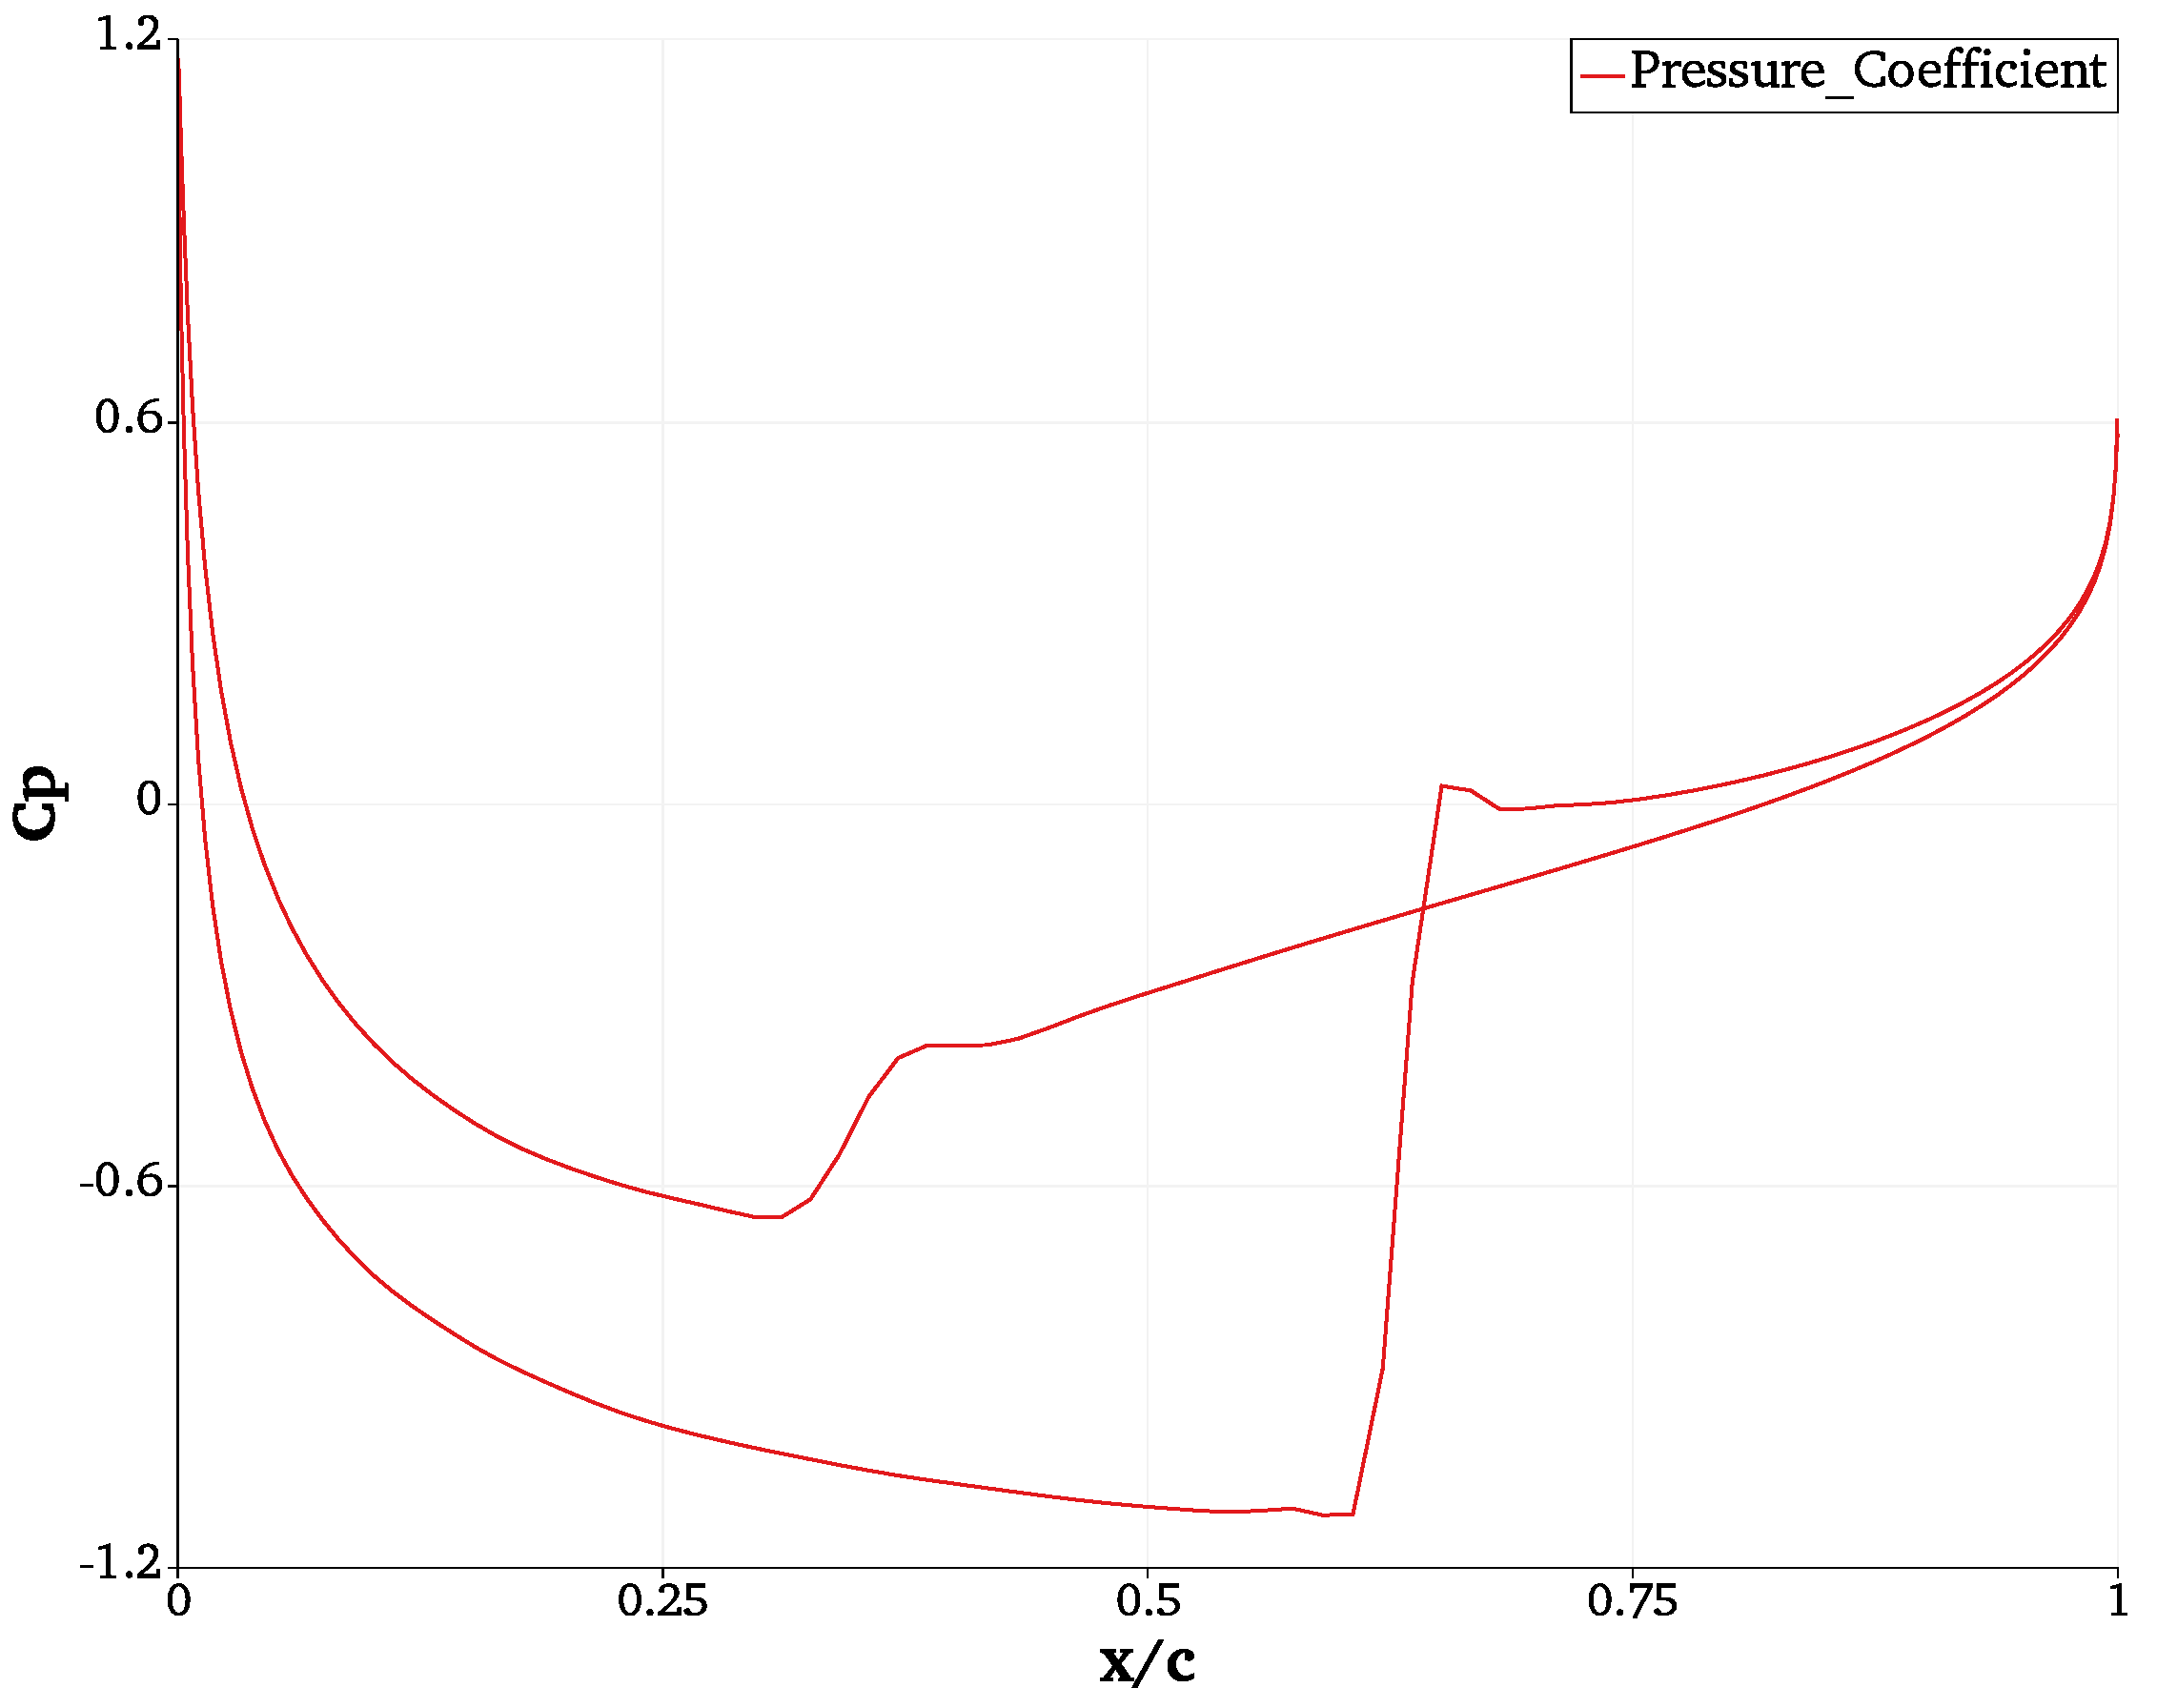
\includegraphics[width=.75\textwidth]{tut01/plot11.pdf}
    \caption{Pressure coefficient on the surface of the NACA0012.}
    \label{fig:surface_pressure}
\end{figure}

Usually $C_p$ is plotted in such a way that the pressure curve in suction side (lower pressure) is on top of the pressure curve on the pressure side (higher pressure). Therefore, we need to reverse  the $y$-axis in the plot (flip). To do this, go to \textbf{Display} from \textbf{Properties} tab. Next, find \textbf{Left Axis Range} section in the same tab, and then click on the \textbf{Left Axis Use Custom Range} (Fig.\ref{fig:viewsetting}). Later, another section appears to select maximum/minimum ranges for left axis of plot. Eventually, just switch numbers in these two text bars. It allows the $y$-axis to be reverse (flipped) as we want it to be.
\begin{figure}[htbp]
    \centering
    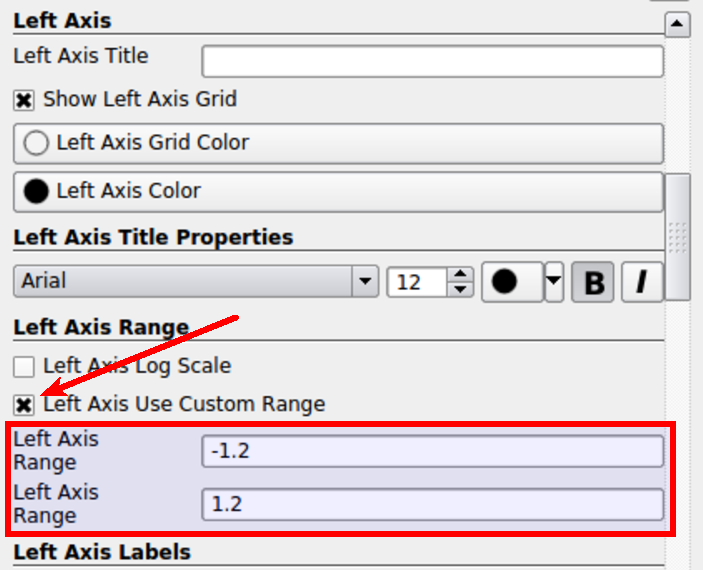
\includegraphics[width=0.5\textwidth]{tut01/leftaxis.pdf}
    \caption{Plot Settings.}
    \label{fig:viewsetting}
\end{figure}
Additionally, there are other parameters that you might change in the same tab, like \textbf{Left Axis Title} or  \textbf{Bottom Axis Title}. To do this, please type $C_p$ and $x/c$ in \textbf{Left Axis Title} and \textbf{Bottom Axis Title}, respectively. Furthermore, for adding marker to the plot lines, form \textbf{Display} select \textbf{Marker Style} as \textit{Diamond} (Fig.\ref{fig:marker}). You can also change the thickness of plot line in the same tab.
\begin{figure}[htbp]
    \centering
    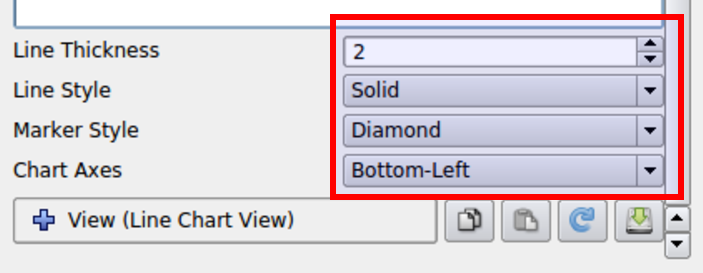
\includegraphics[width=0.4\textwidth]{tut01/addingmarker.pdf}
    \caption{How to add marker to plot.}
    \label{fig:marker}
\end{figure}
Eventually, the final plot you should get is like Fig.\ref{fig:surface_pressure2}
\begin{figure}[htbp]
    \centering
    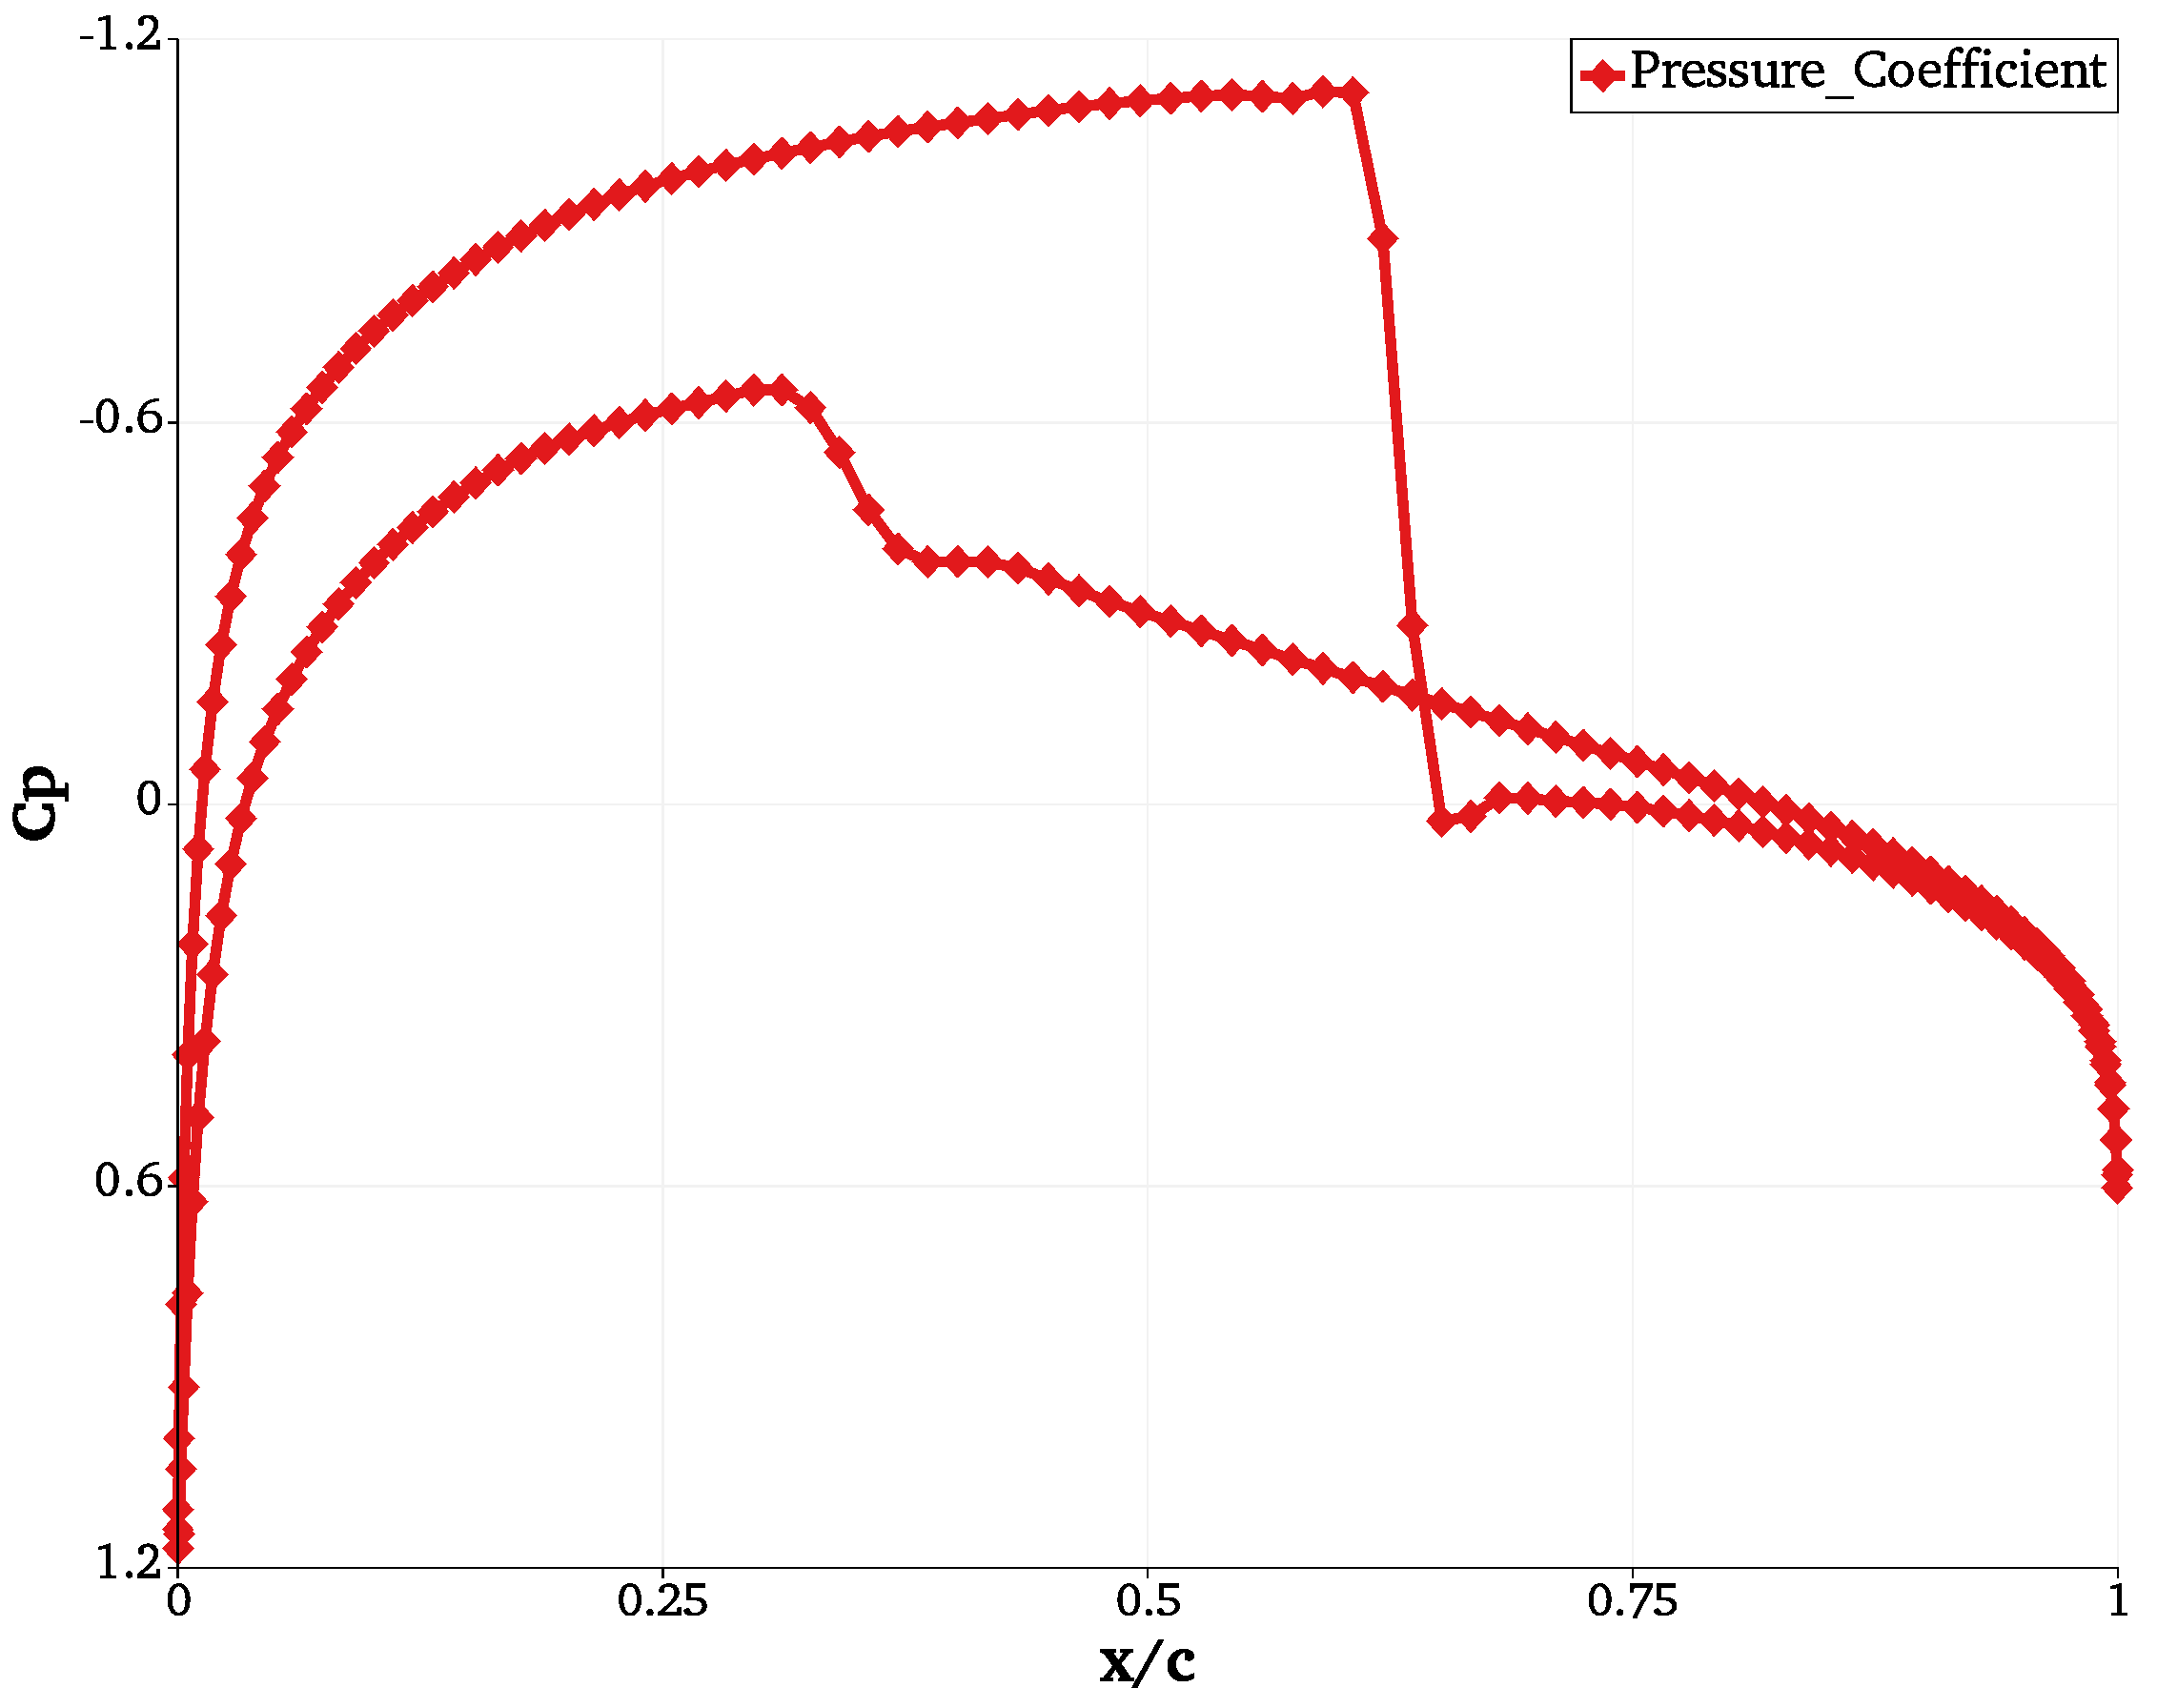
\includegraphics[width=.75\textwidth]{tut01/plot22.pdf}
    \caption{Revised version of the pressure coefficient plot on the surface of the NACA0012.}
    \label{fig:surface_pressure2}
\end{figure}
%--------------------------------------------------------------
\subsection{Forces on the Airfoil}
In order to obtain the aerodynamic loads on the airfoil, open \textit{force\_breakdown}.dat using a text editor software. According to Fig.\ref{fig:forcefile1}, in this file there are flow properties that you can check if the values are the same as those in configuration file. 
\begin{figure}[htbp]
    \centering
    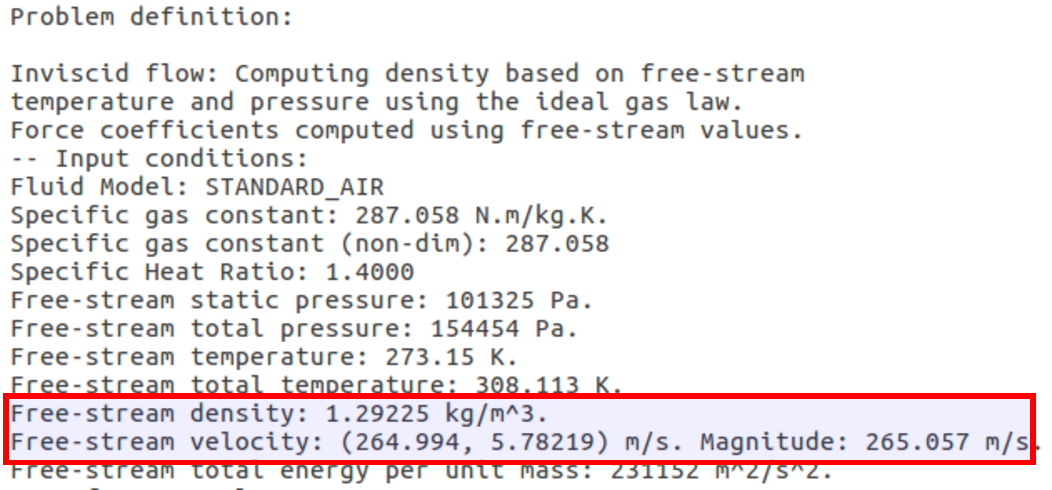
\includegraphics[width=0.9\textwidth]{tut01/forcefile1.pdf}
    \caption{Fluid and flow properties form \textit{force\_breakdown}.dat.}
    \label{fig:forcefile1}
\end{figure}

Additionally, according to Fig.\ref{fig:forcefile2}, the aerodynamic loads are expressed in non-dimensional form by using free-stream values for density and velocity, as well as one reference length (or area). It could be a good practice to check if the non-dimensional factor corresponds to the expected free-stream values. The actual forces (dimensional) can be obtained by multiplying coefficient with non-dimensional factor calculated by free-stream density and velocity. Note that you can find lift coefficient ($C_L$), drag coefficient ($C_D$), lift to drag ratio ($C_L / C_D$), the moment coefficient ($C_{M,z}$), $x$-component of force coefficient ($C_{F,x}$) and $y$-component of force coefficient ($C_{F,y}$) all from the \textit{force\_breakdown}.dat.
\begin{figure}[htbp]
    \centering
    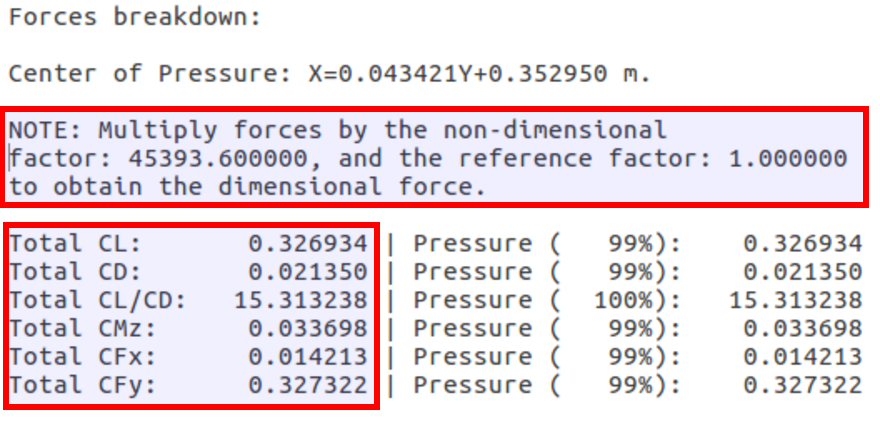
\includegraphics[width=0.8\textwidth]{tut01/forcefile2.pdf}
    \caption{Aerodynamic loads from \textit{force\_breakdown}.dat.}
    \label{fig:forcefile2}
\end{figure}
%++++++++++++++++++++++++++++++++++++++++++++++++++++++++++++++
\section{Questions}
1. Run the provided default NACA0012 test case at the provided Ma = 0.8.
\begin{enumerate}[label=(\alph*)]
    \item Plot and comment on the mesh.
    \item Plot and comment on the pressure contours around the airfoil.
    \item Plot and comment on the pressure coefficient on the surface of the airfoil.
\end{enumerate}
2. Re-run the default NACA0012 case but change the Mach number to Ma = 0.3 and run several simulations using alpha = 0, 2, 4, 6, 8, 10, 12, 14, 16 degrees.
\begin{enumerate}[label=(\alph*)]
    \item Plots Cl vs alpha alongside the provided experimental data \cite{ladson1988effects} in the test case folder.
    \item Repeat 1.b with Ma = 0.3 for the alpha = 0, 8, 16 degree cases.
    \item Repeat 1.c with for the alpha = 0, 8, 16 degree cases and include the provided experimental data  in the \cite{ladson1987pressure}.
\end{enumerate}
3. Compare your CFD results in Question 2). Discuss sources of error that could have led to any discrepancies in your results.
%--------------------------------------------------------------
%++++++++++++++++++++++++++++++++++++++++++++++++++++++++++++++
%++++++++++++++++++++++++++++++++++++++++++++++++++++++++++++++
%++++++++++++++++++++++++++++++++++++++++++++++++++++++++++++++
\chapter{Supersonic Wedge}
%++++++++++++++++++++++++++++++++++++++++++++++++++++++++++++++
\section{Problem Description}
In this tutorial, we are going to explain how to simulate supersonic inviscid flow past a simple 2D wedge. This wedge generates oblique-shock for high Mach number flows. Keep in mind that if the Reynolds number is high enough, the viscosity term in Navier-Stokes equations becomes negligible, and then, flow can be assumed to be inviscid. The another assumption we take is that the flow is a perfect gas. Furthermore, the domain is a structured mesh with 3,750 nodes. The upper wall is a flat Euler wall. The lower wall is also Euler wall with a wedge starting at $x/L=1/3$, where $L$ is the length of duct. Additionally, the wedge angle is 10 degree. For this example, the flow specifications are provided as follows:
\begin{itemize}
    \item Pressure = 101,325 Pa
    \item Temperature = 273.15 K
    \item Mach number = 2.0
    \item Wedge angle = 10 degrees
\end{itemize}
The tutorial has two parts: Flow Solution and Post-processing. In the first part, we explain how to manage prerequisite files and settings, and how to run the CFD simulation using SU2. In the second part, we explain how to use Paraview software to visualize data obtained form SU2.
%++++++++++++++++++++++++++++++++++++++++++++++++++++++++++++++
\section{Flow solution}
To run the simulation, the SU2 needs two essential files: configuration file (.cfg) and mesh file (.su2). In this example, the following files are located in \textit{02InviscidSupersonicWedge} folder:
\begin{enumerate}
    \item inv\_wedge\_HLLC.cfg as a configuration file.
    \item mesh\_wedge\_inv.su2 as a mesh file.
\end{enumerate}
The next step is to copy these two files in directory of SU2, where the execution and script files are located there. To run this simulation, open the command line terminal and enter the following commands:
\begin{table}[htbp]
    \centering
    \begin{tabular}{|l|l|}
    \hline
    Windows     & \begin{tabular}{c} \$ cd "where you saved the package" \\ \$ SU2\_CFD.exe inv\_wedge\_HLLC.cfg \end{tabular}
    \\
    \hline
    OSX     & \begin{tabular}{c} \$ cd "where you saved the package" \\ \$ SU2\_CFD.exe inv\_wedge\_HLLC.cfg \end{tabular}
    \\
    \hline
    \end{tabular}
\end{table}

The SU2 solver will commence calculation and print out the residuals at every iteration until the specified convergence criteria is achieved. After calculations are done, the following output files should be generated and saved in the SU2 folder:
\begin{itemize}
    \item \textit{flow}.vtk: contains the full volume flow solution.
    \item \textit{force\_breakdown}.dat: contains forces and moment on the surface of the duct.
    \item \textit{history}.vtk: contains convergence history of calculations.
    \item \textit{restart\_flow}.dat: for restarting simulation.
    \item \textit{surface\_flow}.vtk: flow solution on the surface of the duct.
    \item \textit{surface\_flow}.csv: comma separated values of flow solution on the surface of the duct (If you want to plot data in another software, like Microsoft Excel, you can use this file).
\end{itemize}
Please keep in mind that every time you run SU2, the output data will be overwritten. Hence, before launching new simulation, you could make a new folder and transfer your data from previous simulation to this folder.
%++++++++++++++++++++++++++++++++++++++++++++++++++++++++++++++
\section{Post-processing}
In this section, we explain how to use Paraview to visualize CFD data for this example. First of all, install Paraview (this tutorial uses Paraview 3.12.0) if you do not have it on your computer. Otherwise, take following steps for visualization:
%--------------------------------------------------------------
\subsection{Load Solution File:}
Launch Paraview. Go to \textbf{File} $\rightarrow$ \textbf{Open}, and then select \textit{flow}.vtk file. On the left side of Paraview window you will see the file appears in \textbf{Pipeline Browser}, under \textbf{builtin}. Now press \textbf{Apply} button in \textbf{Properties} tab, just right under the  \textbf{Pipeline Browser}. After taking these steps, your file is loaded by software and is ready to visualize (Fig.\ref{fig:load}).
\begin{figure}[htbp]
    \centering
    \includegraphics[width=0.4\textwidth]{tut02/loadvtkfile.pdf}
    \caption{Loading .vtk file in the \textbf{Pipeline Browser}.}
    \label{fig:load}
\end{figure}
%--------------------------------------------------------------
\subsection{Visualize Mesh Domain}
According to Fig.\ref{fig:wireframe}, in order to view mesh, select \textit{Solid Color} with \textit{Wireframe} in the toolbar. Then, you can even zoom in to see mesh for wedge domain, like Fig.\ref{fig:mesh}. As you can see, the mesh in the duct is structured, and at some point the wedge changes the direction of mesh in domain. Additionally, the grids are approximately uniform in whole domain without any significant clustering.
\begin{figure}[htbp]
    \centering
    \includegraphics[width=0.6\textwidth]{tut02/wireframe.pdf}
    \caption{How to display mesh in computational domain.}
    \label{fig:wireframe}
\end{figure}
\begin{figure}[htbp]
    \centering
    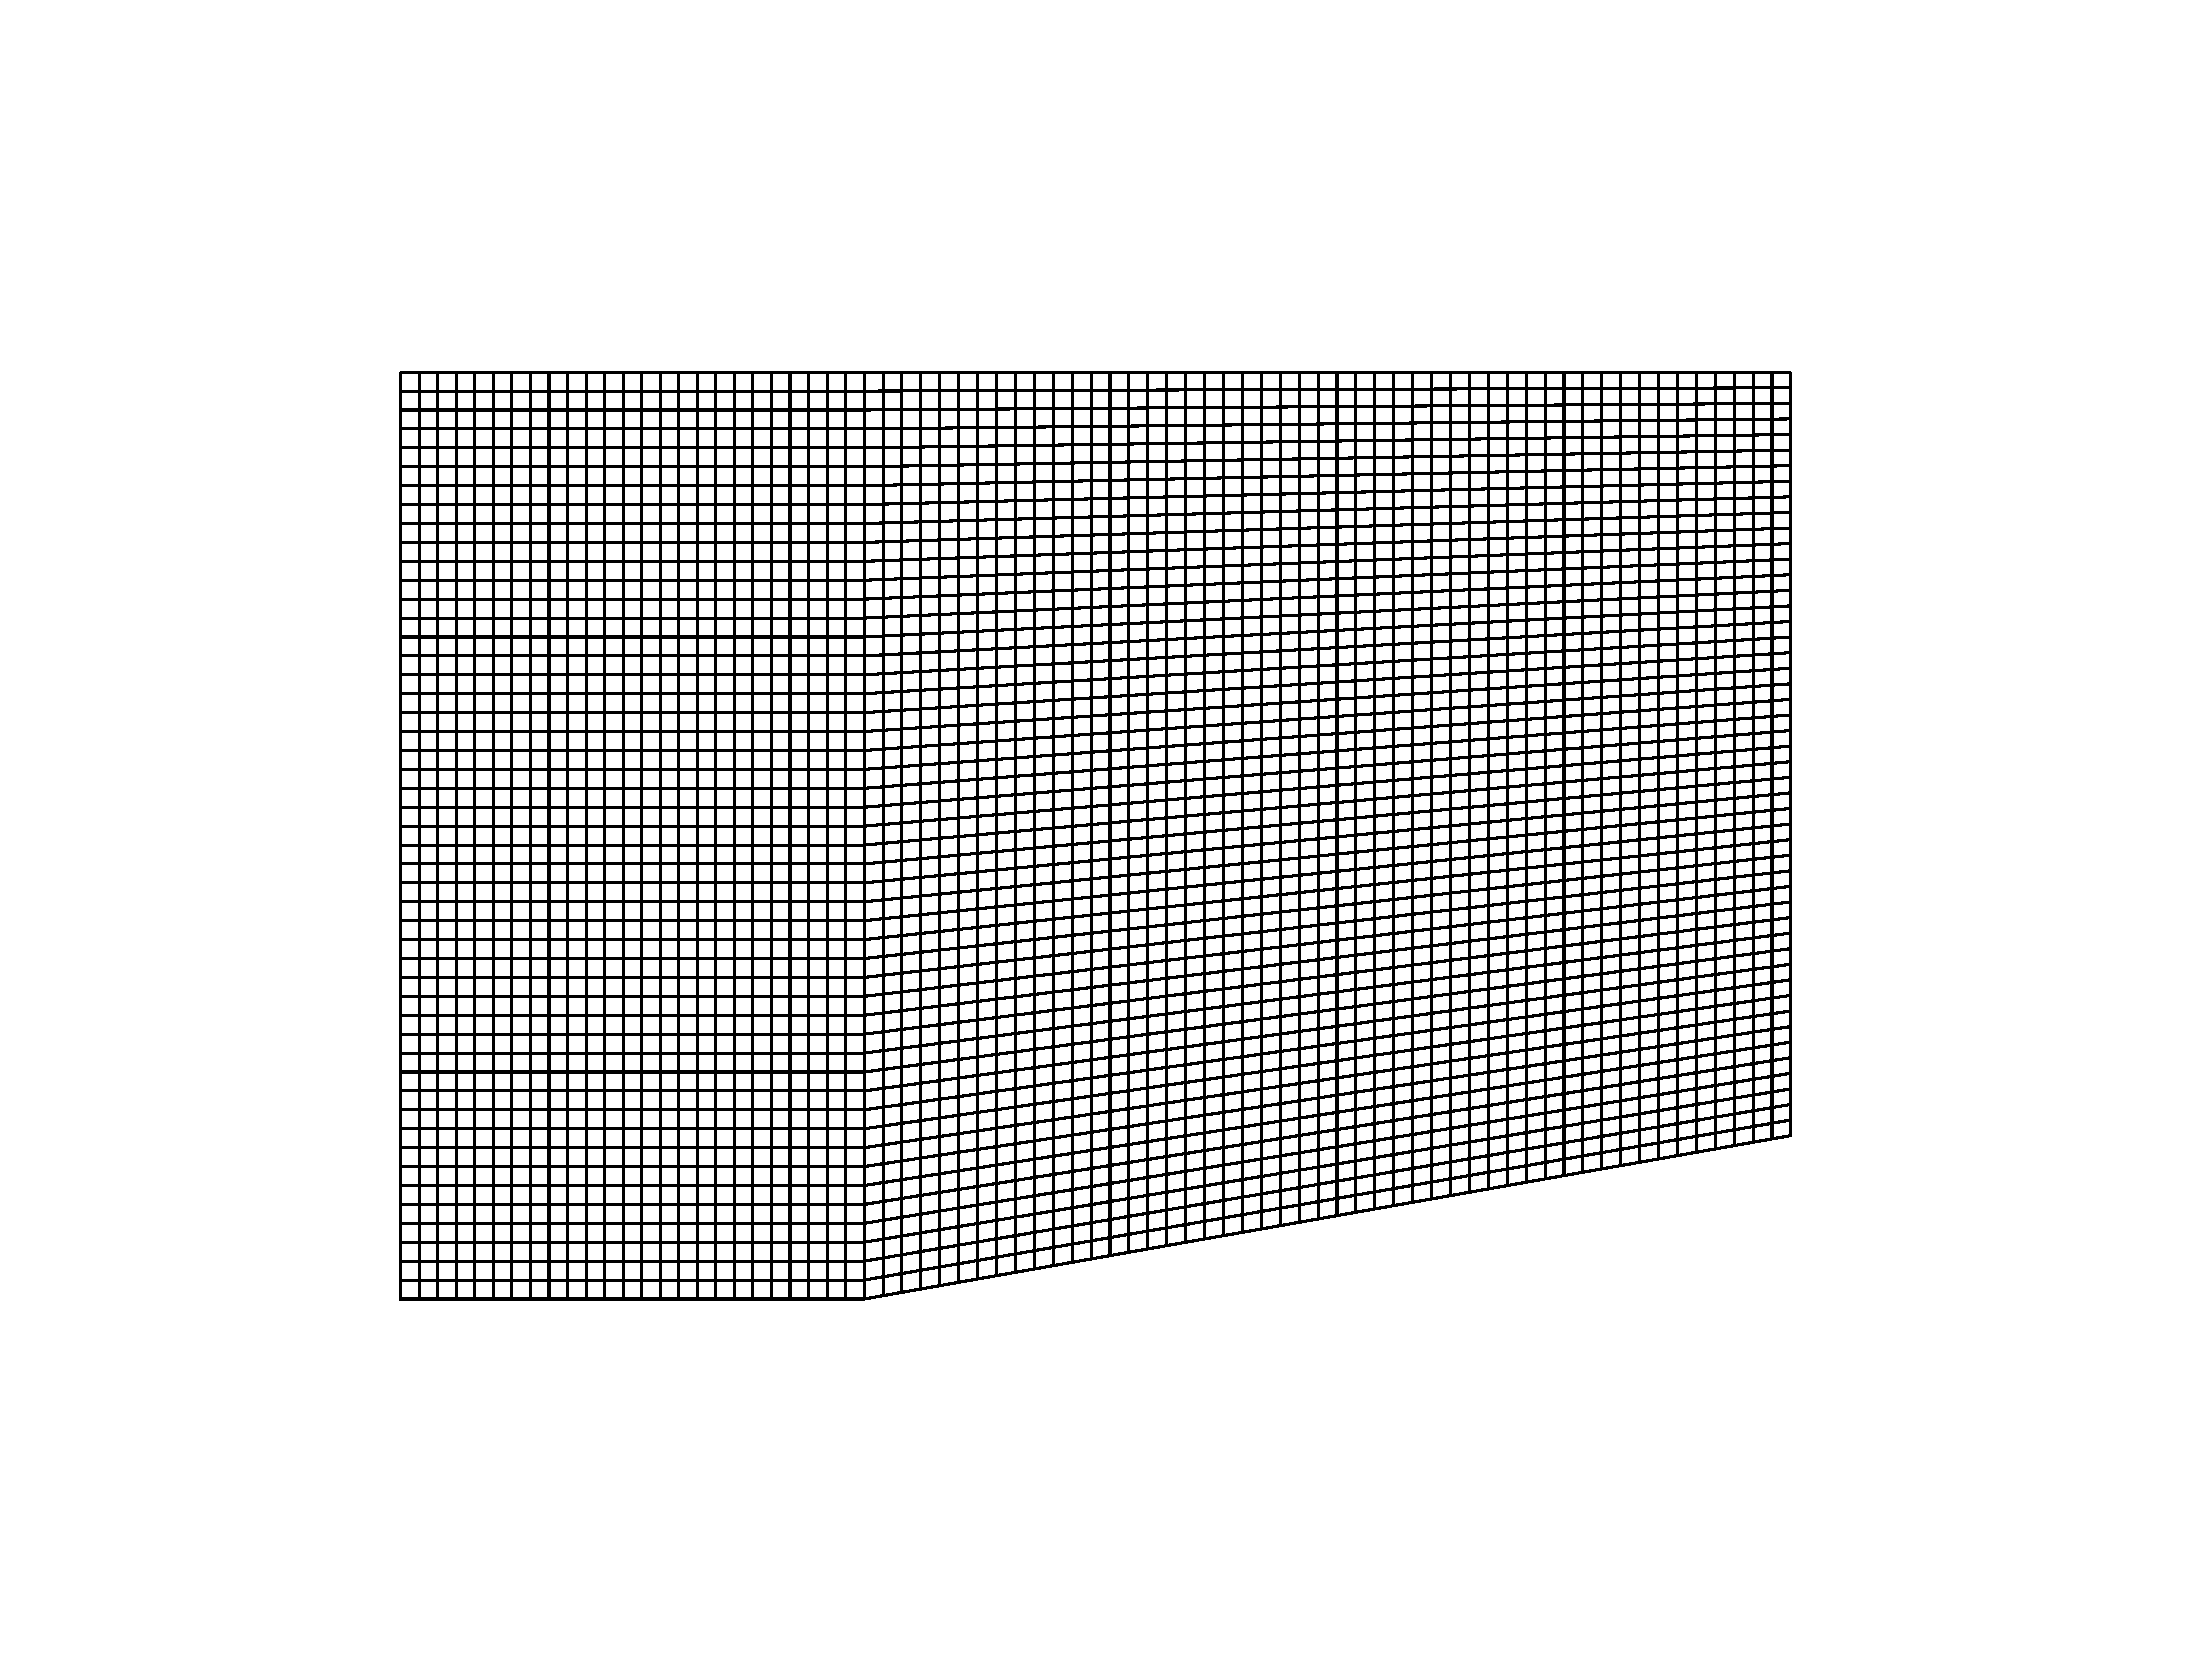
\includegraphics[width=.75\textwidth]{tut02/mesh.pdf}
    \caption{Structured mesh for wedge domain.}
    \label{fig:mesh}
\end{figure}
%--------------------------------------------------------------
\subsection{Visualize Pressure Contour and Mach Contour}
To display the pressure contour, click on the \textit{flow}.vtk in \textbf{Pipeline Browser} to activate the file, and then click on \textbf{Display} form \textbf{Properties} tab. Under \textbf{Coloring} section, select \textit{Pressure} from drop-down menu (Fig.\ref{fig:pressure contours setting}). Additionally, for changing color settings for the pressure, you can click on the \textbf{Edit} under the \textbf{Coloring}.
\begin{figure}[htbp]
    \centering
    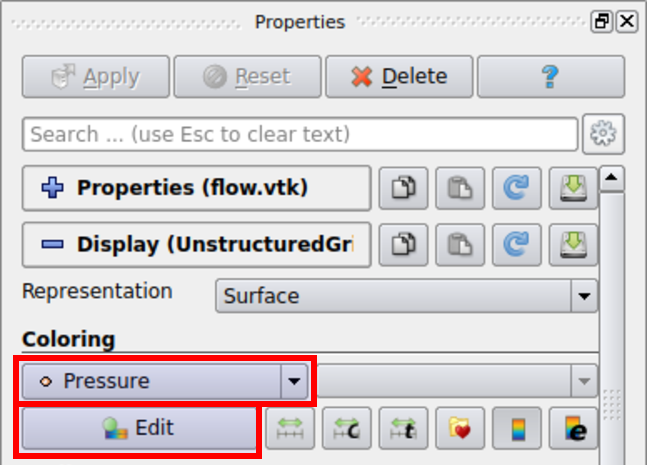
\includegraphics[width=0.4\textwidth]{tut02/pressurecont.pdf}
    \caption{Settings for displaying the pressure contour.}
    \label{fig:pressure contours setting}
\end{figure}
Normally, another display window appears on the right-hand side of the monitor, named as \textbf{Mapping Data}, similar to Fig.\ref{fig:color_range}.
\begin{figure}[htbp]
    \centering
    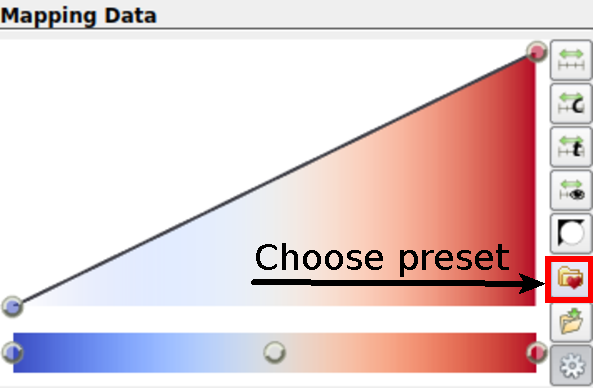
\includegraphics[width=0.4\textwidth]{tut02/colorrange.pdf}
    \caption{Changing color range for pressure contour.}
    \label{fig:color_range}
\end{figure}
Now you can change contour colors by choosing \textbf{Choose preset}. Here, we select \textit{Cold and Hot} color range to be able to show clearly the sharp changes in pressure values (Fig.\ref{fig:color_range_item}). Then, click \textbf{Apply} for the next step.
\begin{figure}[htbp]
    \centering
    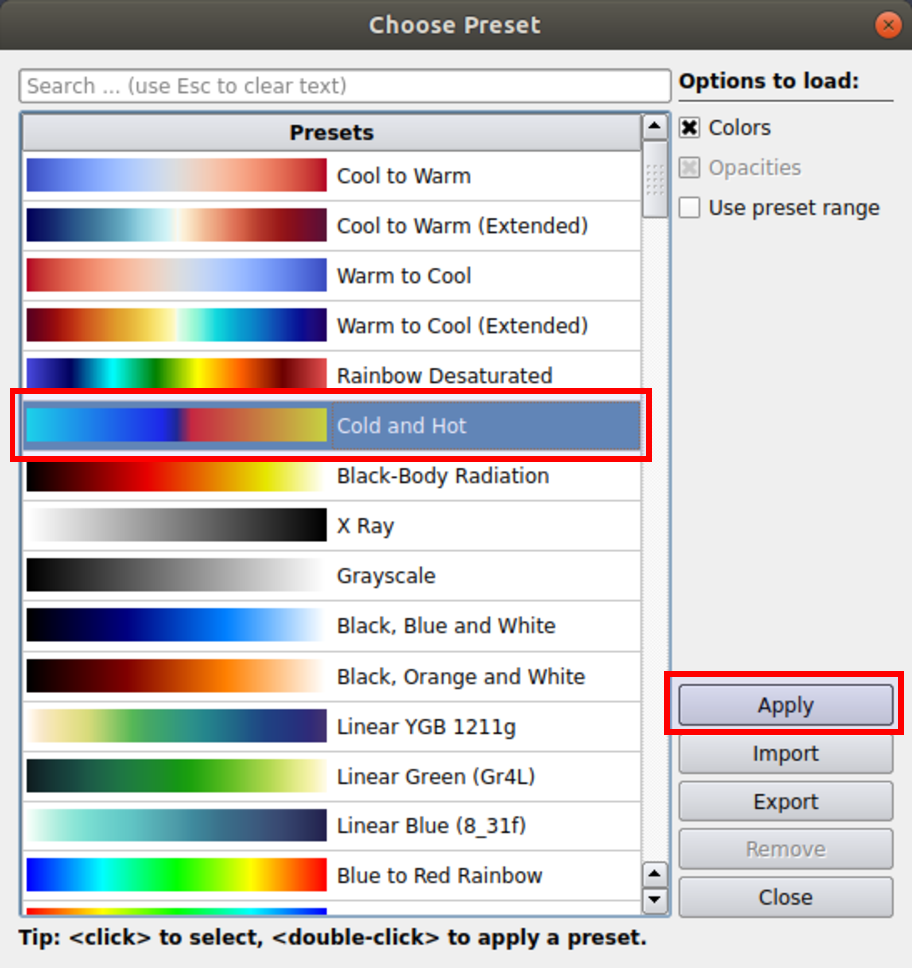
\includegraphics[width=0.5\textwidth]{tut02/changecontourcolors.pdf}
    \caption{Different color ranges to display contour.}
    \label{fig:color_range_item}
\end{figure}
Additionally, to add axis to plots, under \textbf{Miscellaneous} form \textbf{Display} (Fig.\ref{fig:add axis}), you can check box beside \textbf{Data Axes Grid}, and then go to \textbf{Edit} and change more options based on your preferences (Fig.\ref{fig:axis setting}).
\begin{figure}[htbp]
    \centering
    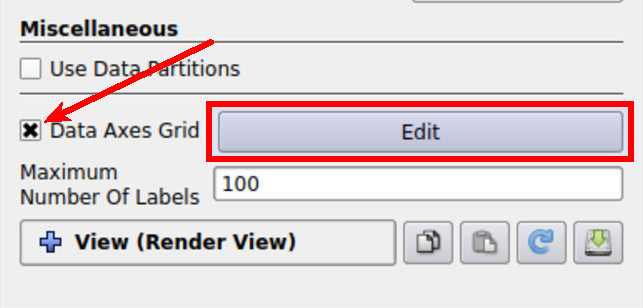
\includegraphics[width=0.4\textwidth]{tut02/addaxis.pdf}
    \caption{How to add axis to the plots.}
    \label{fig:add axis}
\end{figure}
\begin{figure}[htbp]
    \centering
    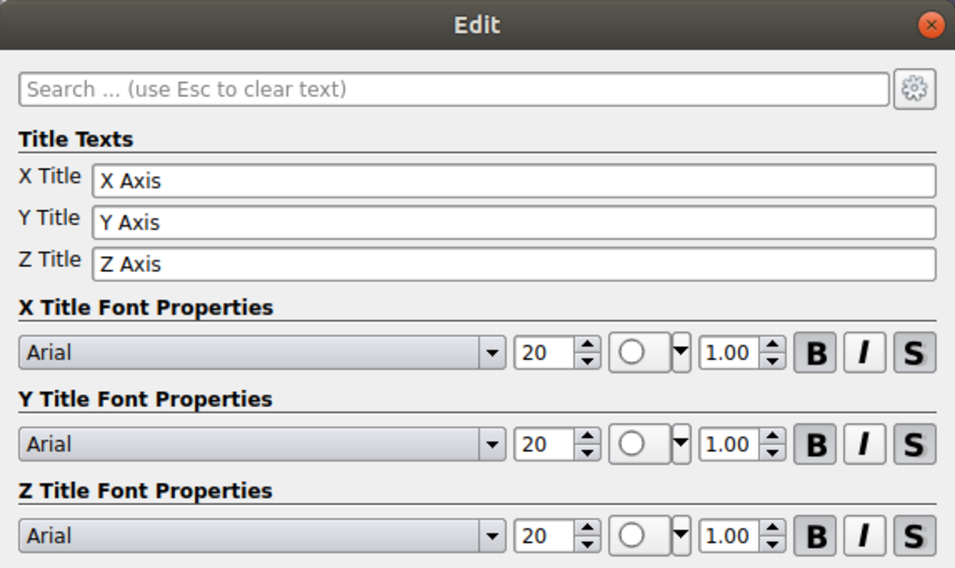
\includegraphics[width=0.6\textwidth]{tut02/axissettings.pdf}
    \caption{Settings for axis style.}
    \label{fig:axis setting}
\end{figure}
Finally, the pressure contour you get should be similar to Fig.\ref{fig:plot pressure cont1}.
\begin{figure}[htbp]
    \centering
    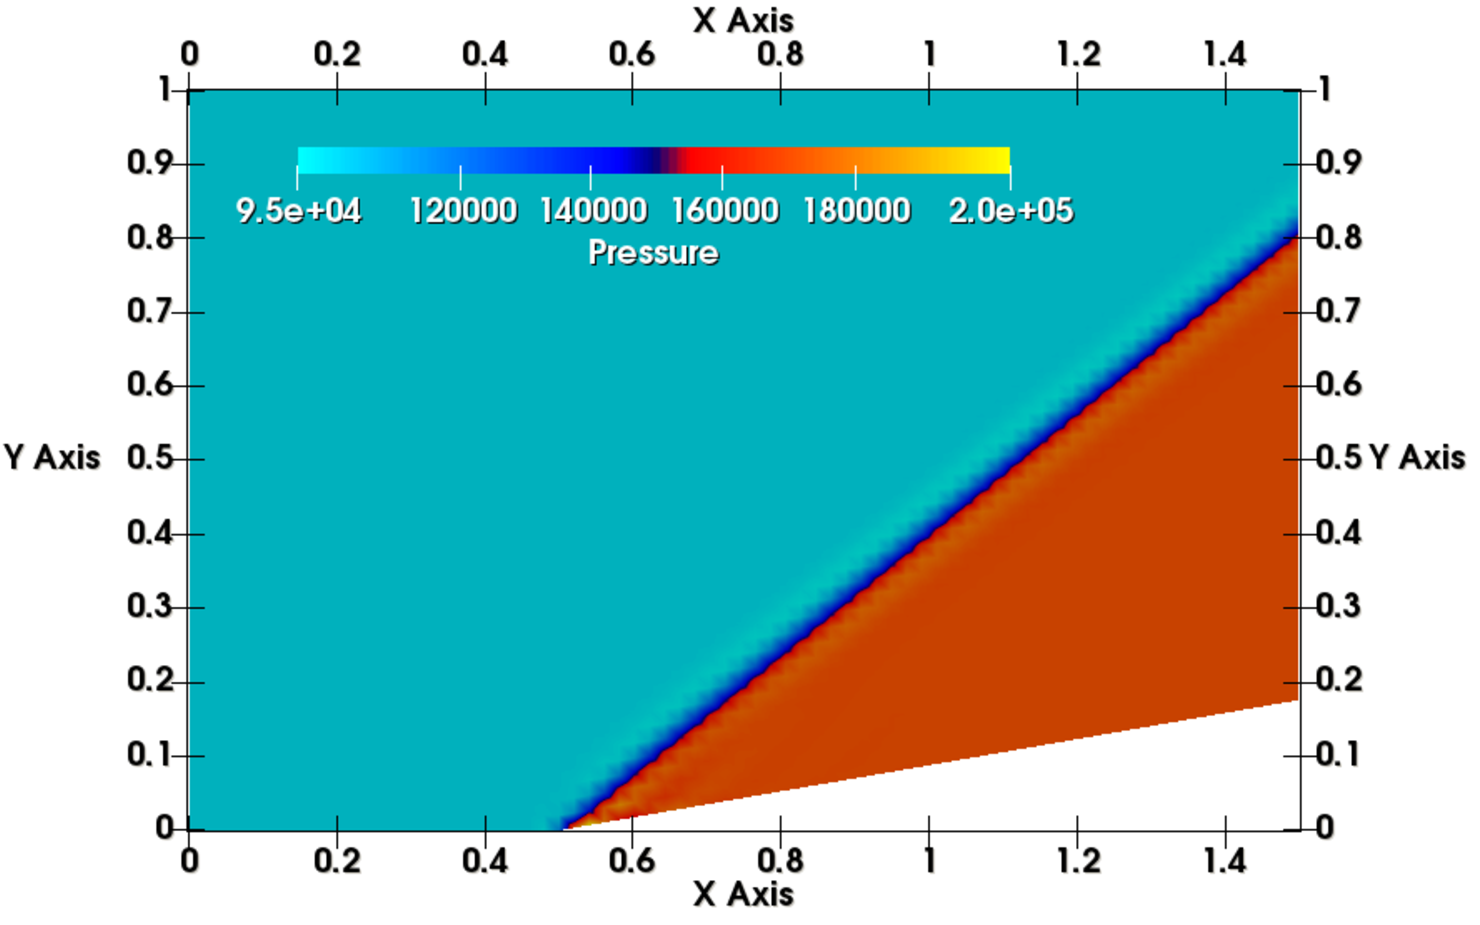
\includegraphics[width=0.85\textwidth]{tut02/plot1pressurecont.pdf}
    \caption{Pressure contour for supersonic wedge.}
    \label{fig:plot pressure cont1}
\end{figure}
%----------------------------------------------------------

The pressure gradient along the shock wave is very difficult to see, and we want to add contour lines to
separate the pressure color gradient. To add contour lines, click again on the \textit{flow}.vtk file in the \textbf{Pipeline Browser}, and then click on the \textbf{Contour} icon (Fig.\ref{fig:contour_icon}) in toolbar.
\begin{figure}[htbp]
    \centering
    \includegraphics[width=0.5\textwidth]{tut02/contourlineicon.pdf}
    \caption{\textbf{Contour} icon in toolbar.}
    \label{fig:contour_icon}
\end{figure}
Eventually,\textit{Contour1} appears under \textit{flow}.vtk file in the \textbf{Pipeline Browser} (Fig.\ref{fig:contour1}). Then, click on \textbf{Apply} to proceed next step.
\begin{figure}[htbp]
    \centering
    \includegraphics[width=0.4\textwidth]{tut02/contour1.pdf}
    \caption{Adding \textit{Contour1} in \textbf{Pipeline Browser}.}
    \label{fig:contour1}
\end{figure}
With regard to Fig.\ref{fig:contourby a}, go to the \textbf{Properties} tab, and select \textit{Pressure} from \textbf{Contour By} drop-down menu. Next, click on the \textbf{Add Range} icon to customize the range of pressure contour. In Fig.\ref{fig:contourby b}, you will see the max/min range of contour lines (i.e. \textbf{From}/\textbf{To}), as well as number of lines you would rather to have in your contour plot (i.e. \textbf{Steps}). Next, set \textbf{Step} to 20, and click \textbf{OK}. By doing this, it means the pressure contour range is equally divided by 20 portions, and the pressure values in each portion are limited by two lines in the display window. At the end, click on \textbf{Apply} to see contour lines in display window.
\begin{figure}[htbp]
    \centering
     \begin{subfigure}[b]{.4\textwidth}
         \centering
         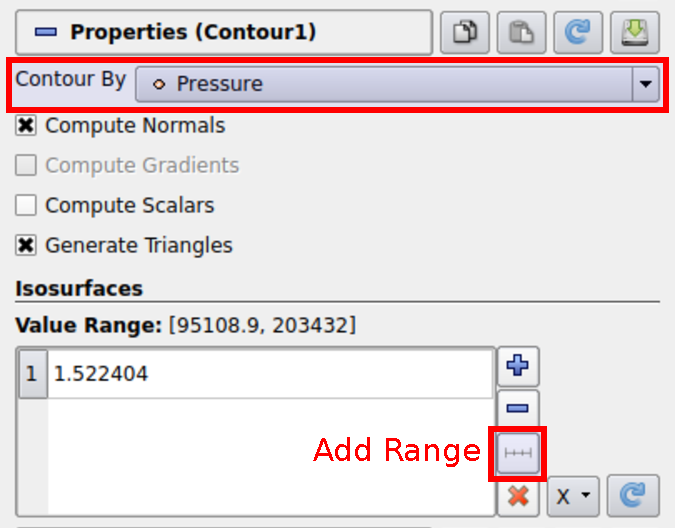
\includegraphics[width=1.0\textwidth]{tut02/contourby.pdf}
         \caption{Define new range}
         \label{fig:contourby a}
     \end{subfigure}
     \hfill
     \begin{subfigure}[b]{.4\textwidth}
         \centering
         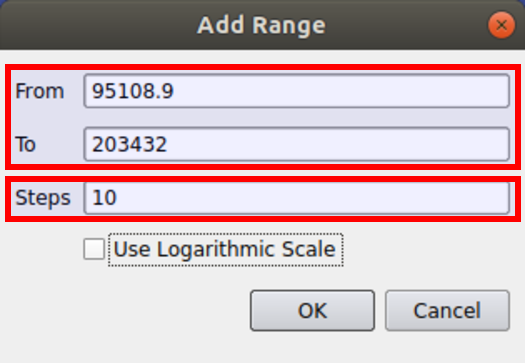
\includegraphics[width=1.0\textwidth]{tut02/addrange.pdf}
         \caption{Add range}
         \label{fig:contourby b}
     \end{subfigure}     
    \caption{How to define a new range for the contour lines.}
    \label{fig:contourby}
\end{figure}
Next, as it is shown in Fig.\ref{fig:colorby2}, click on the \textbf{Display} under \textbf{Properties} tab. In \textbf{Coloring} section, select \textbf{Solid Color} form drop-down menu, and choose white color form \textbf{Edit}.
\begin{figure}[htbp]
    \centering
    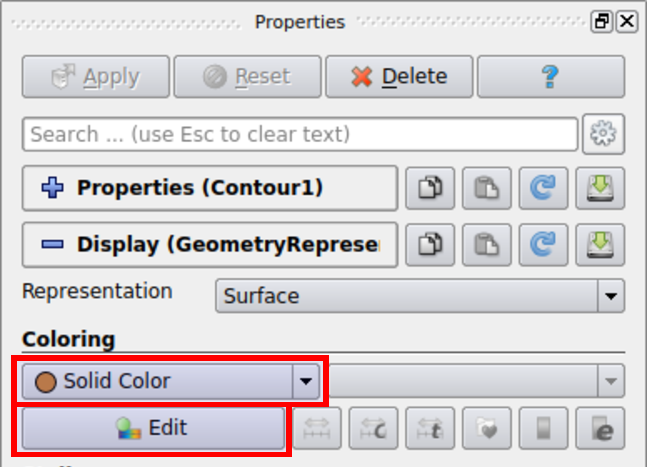
\includegraphics[width=0.4\textwidth]{tut02/contourline.pdf}
    \caption{Changing contour lines color in \textbf{Coloring} section.}
    \label{fig:colorby2}
\end{figure}
Eventually, the pressure contour with contour lines should be similar to Fig.\ref{fig:pressure_contour_lines}.
\begin{figure}[htbp]
    \centering
    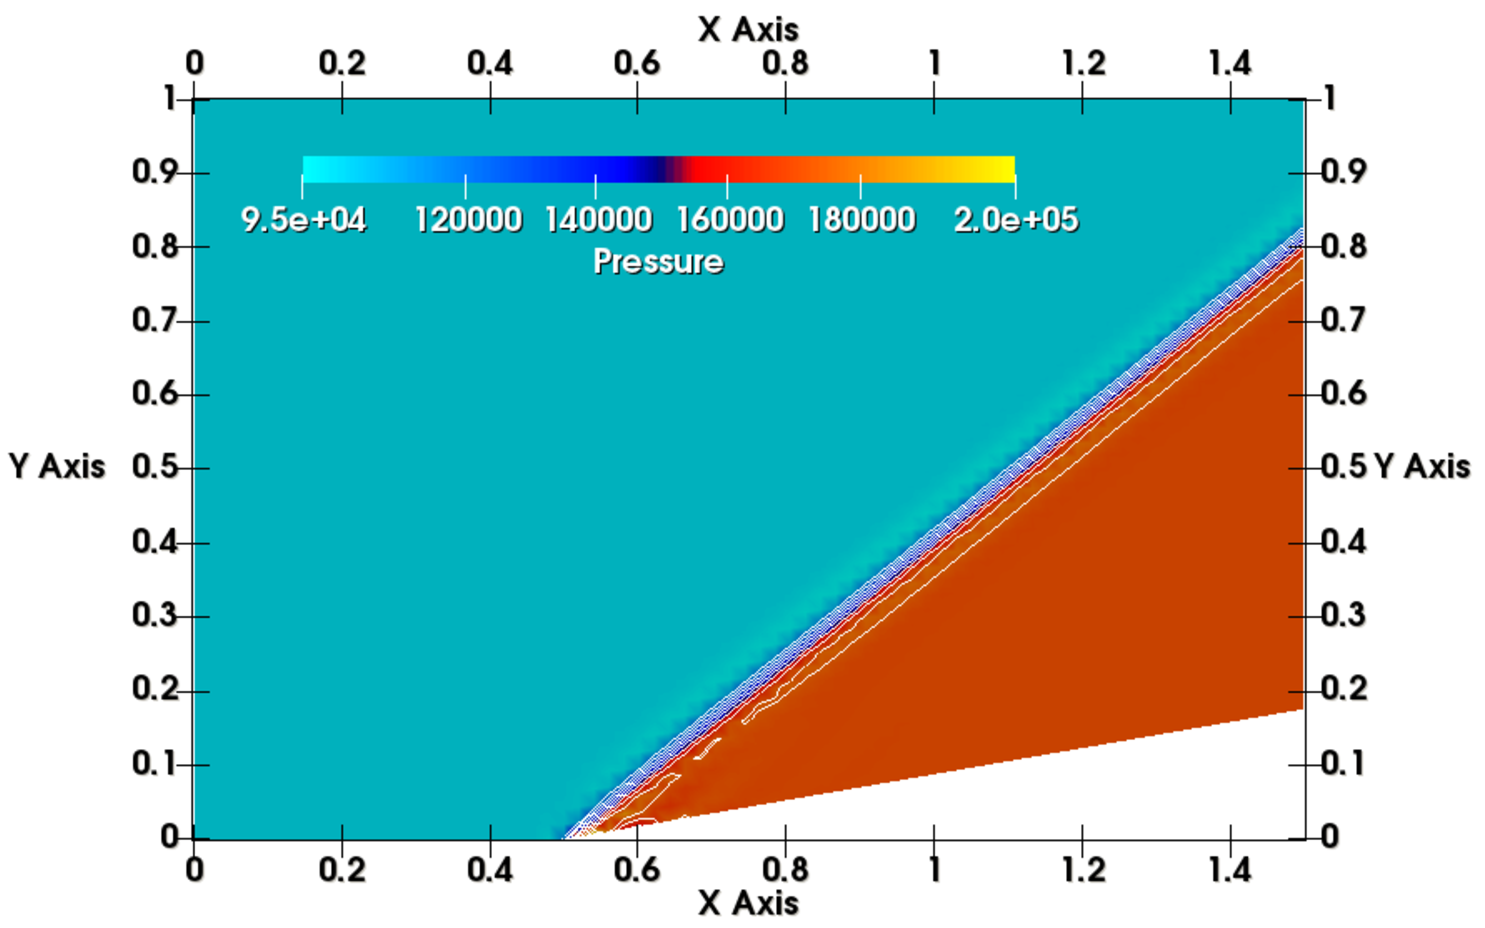
\includegraphics[width=.85\textwidth]{tut02/plot2pressurecont.pdf}
    \caption{Pressure contour superimposed by contour lines for supersonic wedge.}
    \label{fig:pressure_contour_lines}
\end{figure}
You can zoom-in to the region at the bottom of the wedge to see the pressure gradient along the oblique
shock, like Fig.\ref{fig:pressure_contour_lines_zoom}.
\begin{figure}[htbp]
    \centering
    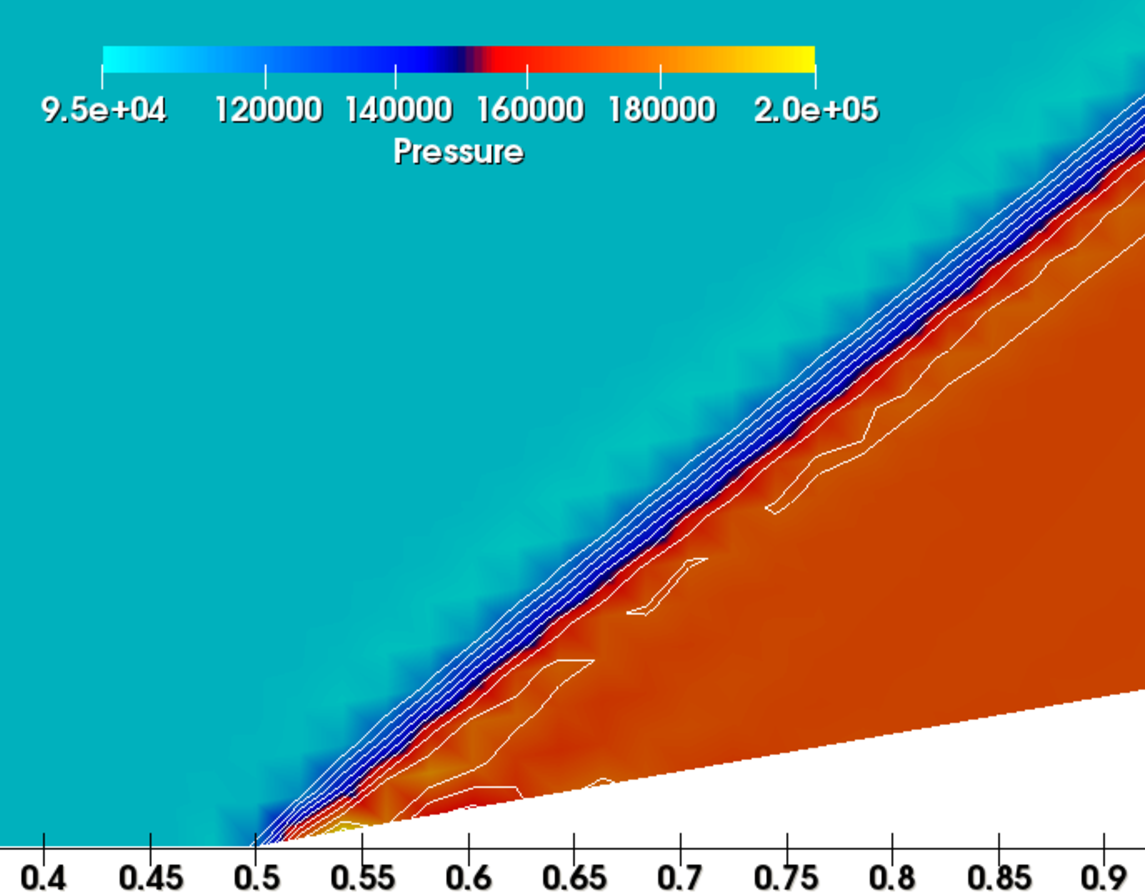
\includegraphics[width=.65\textwidth]{tut02/plot3pressurecont.pdf}
    \caption{Magnified pressure contour superimposed by contour lines for supersonic wedge.}
    \label{fig:pressure_contour_lines_zoom}
\end{figure}

The other important plot we want to show is related to Mach number contour. To display the Mach number contour, click on \textit{flow}.vtk in the \textbf{Pipeline Browser}. Similar to Fig.\ref{fig:pressure contours setting}, under \textbf{Coloring} section, select \textit{Mach} from drop-down menu. Next, click on \textit{Contour1} in the \textbf{Pipeline Browser}. Later, under \textbf{Properties}, select \textit{Mach} from \textbf{Contour By} drop-down menu. Since all the settings are related to pressure value, we need to revise some options for \textit{Mach} value. To do this, first of all, we need to delete data range for pressure and replace it with data range of Mach number. Under \textbf{Isosurfaces} from \textbf{Properties}, click on the \textbf{Remove All} icon, and then click on the \textbf{Add Range} icon, as shown in Fig.\ref{fig:contourby2 a}. As you can see form Fig.\ref{fig:contourby2 b}, the max/min values for mach number has changed. Now set the \textbf{Steps} to 20 and click on \textbf{OK} to proceed next step.
\begin{figure}[htbp]
    \centering
     \begin{subfigure}[b]{.4\textwidth}
         \centering
         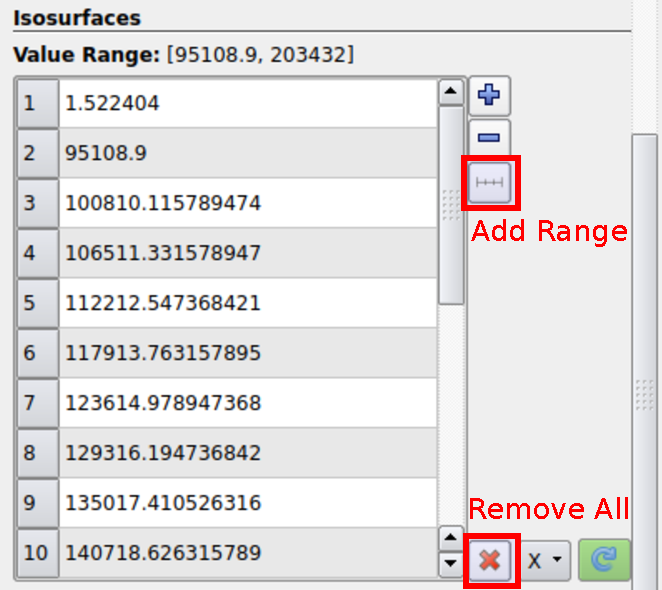
\includegraphics[width=1.0\textwidth]{tut02/deladdrange.pdf}
         \caption{Define new range}
         \label{fig:contourby2 a}
     \end{subfigure}
     \hfill
     \begin{subfigure}[b]{.4\textwidth}
         \centering
         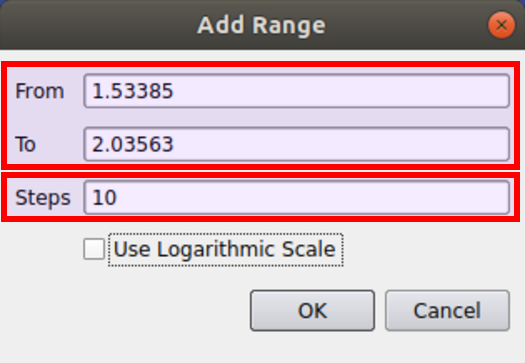
\includegraphics[width=1.0\textwidth]{tut02/addrange2.pdf}
         \caption{Add range}
         \label{fig:contourby2 b}
     \end{subfigure}     
    \caption{How to define a new range for the contour lines.}
    \label{fig:contourby2}
\end{figure}
Now the Mach number contour should look like Fig.\ref{fig:mach_contour}. Additionally, if you zoom-in the plot, you will see more contour details near the wedge similar to Fig.\ref{fig:mach_contour_zoom}.
\begin{figure}[htbp]
    \centering
    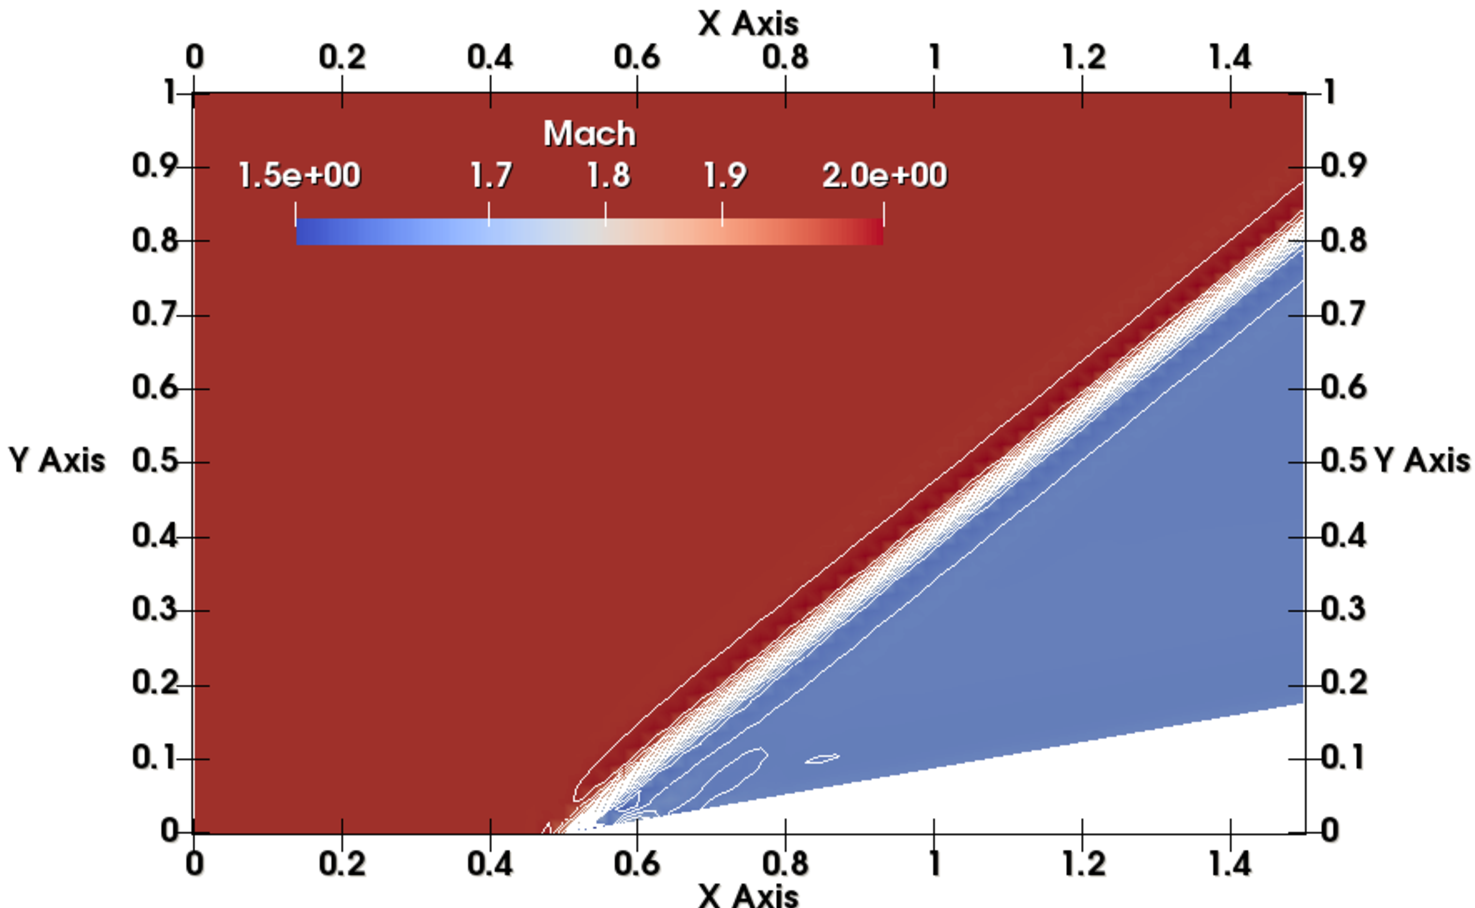
\includegraphics[width=.85\textwidth]{tut02/plot1machcont.pdf}
    \caption{Mach number contour superimposed by contour lines for supersonic wedge.}
    \label{fig:mach_contour}
\end{figure}
\begin{figure}[htbp]
    \centering
    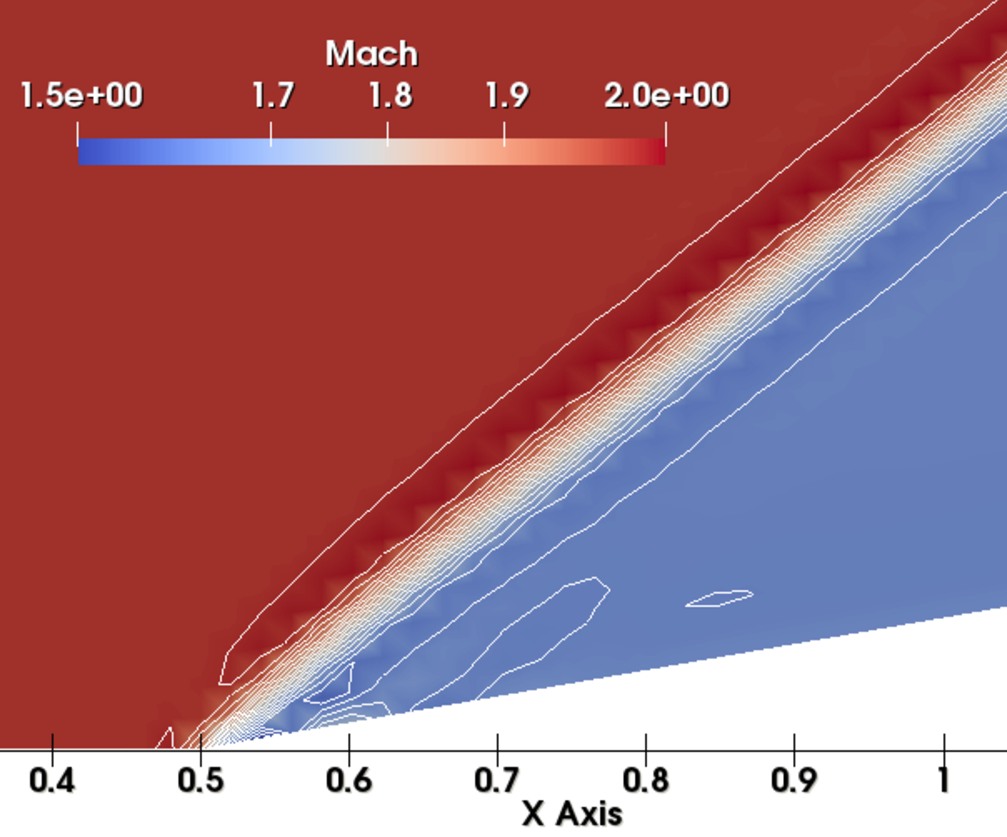
\includegraphics[width=.65\textwidth]{tut02/plot1machcont2.pdf}
    \caption{Magnified Mach number contour superimposed by contour lines for supersonic wedge.}
    \label{fig:mach_contour_zoom}
\end{figure}
%--------------------------------------------------------------
\subsection{Plotting a variable over an arbitrary line}
For plotting variable over an arbitrary line, you can activate \textit{flow}.vtk by clicking on it in the \textbf{Pipeline Browser}. Next, as shown in Fig.\ref{fig:plot_over_line}, go to \textbf{Filters} $\rightarrow$  \textbf{Data Analysis} $\rightarrow$  \textbf{Plot Over Line}.
\begin{figure}[htbp]
    \centering
    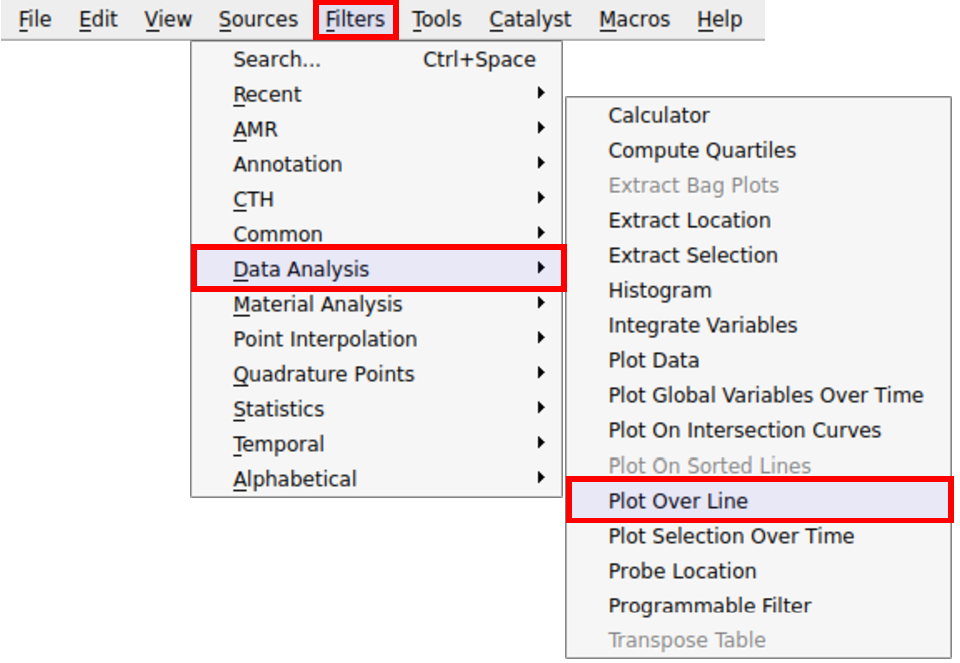
\includegraphics[width=.75\textwidth]{tut02/plotoverline.pdf}
    \caption{How to plot over an arbitrary line.}
    \label{fig:plot_over_line}
\end{figure}
Next, according to Fig.\ref{fig:line_coordinate}, under \textbf{Line Parameters} from \textbf{Properties}, select the coordinates for two arbitrary points you want (i.e. \textbf{Point1} and \textbf{Point2}). In this case, plot the line from \textbf{Point1} to \textbf{Point2} with (0,0.5,0) and (1.5,0.5,0), respectively, and then, click on \textbf{Apply}.
\begin{figure}[htbp]
    \centering
    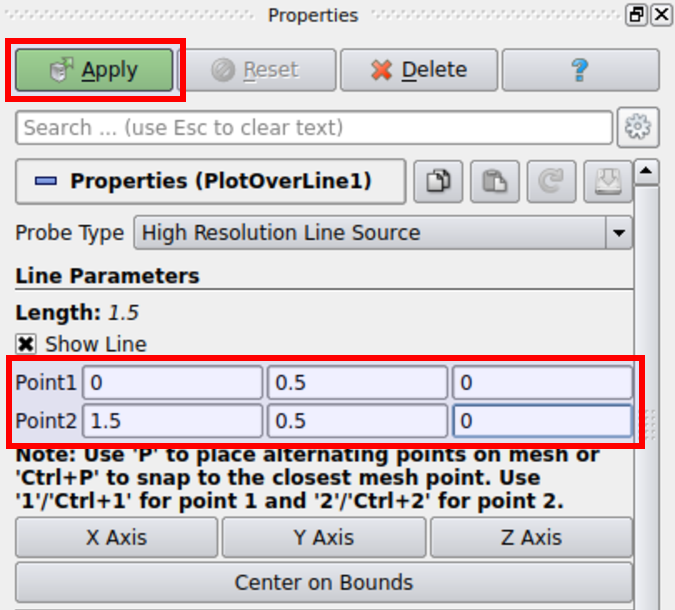
\includegraphics[width=.45\textwidth]{tut02/linecoord.pdf}
    \caption{Define the coordinates for plotting over the line.}
    \label{fig:line_coordinate}
\end{figure}
Eventually, a plot will be generated. According to Fig.\ref{fig:plot_line_setting}, under \textbf{X Axis Parameters} from \textbf{Display}, pick \textit{Point\_X} from \textbf{X Array Name} drop-down menu. Furthermore, under \textbf{Series Parameters}, toggle the box beside \textbf{Variable} to uncheck everything, then select the \textit{Mach} among all variables existed.
\begin{figure}[htbp]
    \centering
    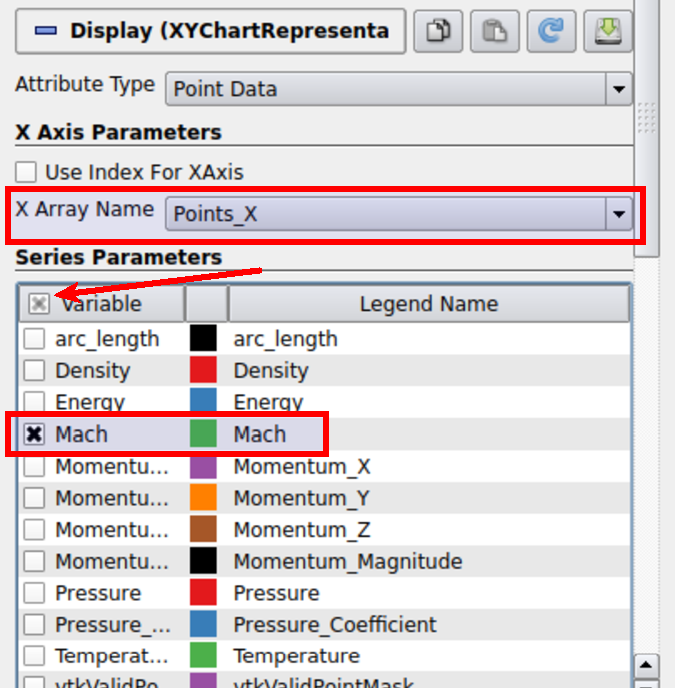
\includegraphics[width=.45\textwidth]{tut02/plotmachline.pdf}
    \caption{How to plot Mach number over a line.}
    \label{fig:plot_line_setting}
\end{figure}
The plot of Mach number vs the \textit{x-coordinate} will be displayed in main window like Fig.\ref{fig:plot_line}.
\begin{figure}[htbp]
    \centering
    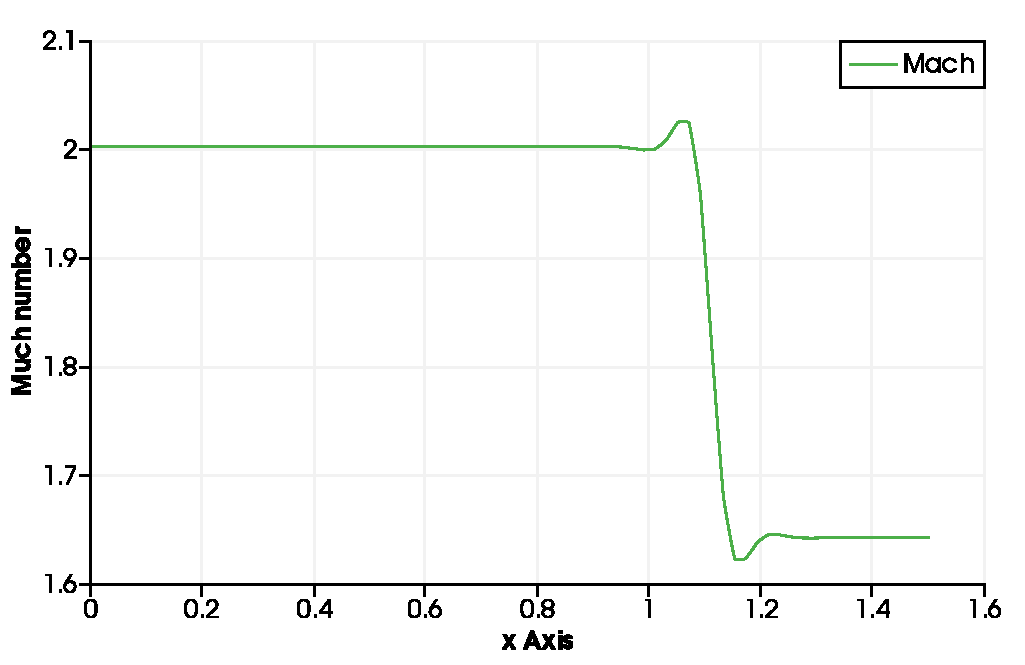
\includegraphics[width=.85\textwidth]{tut02/plot2contourline.pdf}
    \caption{Mach number plot over a specified line in \textit{x-coordinate}.}
    \label{fig:plot_line}
\end{figure}
In order to see the spreadsheet view, click the upper right icon as shown in Fig.\ref{fig:open_spreadsheet}, then click on the \textit{Spreadsheet View} like Fig.\ref{fig:spreadsheet}.
\begin{figure}[htbp]
    \centering
    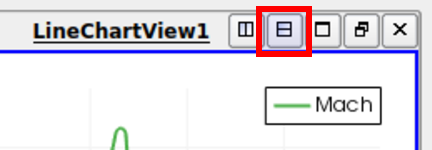
\includegraphics[width=.3\textwidth]{tut02/openspreadsheet.pdf}
    \caption{How to make spreadsheet view in a new window.}
    \label{fig:open_spreadsheet}
\end{figure}
\begin{figure}[htbp]
    \centering
    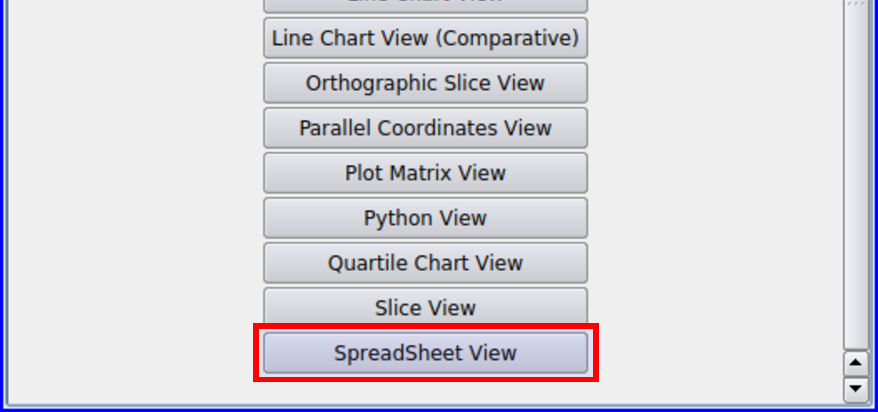
\includegraphics[width=.65\textwidth]{tut02/spreadsheet.pdf}
    \caption{Selecting \textit{Spreadsheet View} among different views.}
    \label{fig:spreadsheet}
\end{figure}
Additionally, you can save .csv file and plot it with other available software such as Microsoft Excel. To export the spreadsheet as a .csv file, go to \textbf{File} $\rightarrow$ \textbf{Export}, and then \textbf{Save as} .csv.
%++++++++++++++++++++++++++++++++++++++++++++++++++++++++++++++
\section{Questions}
1. Run the default case as provided which uses 2ND\_ORDER and the HLLC Riemann solver.
\begin{enumerate}[label=(\alph*)]
    \item Create coloured contours of Pressure and Mach number in the entire domain.
    \item Plot Pressure from (0,0.5,0) to (1.5,0.5,0) using the \textbf{Plot Over Line}.
\end{enumerate}
2. Repeat Q.1 but switch the SPATIAL\_ORDER\_FLOW to 1ST\_ORDERs. \\
3. Repeat 1 using SPATIAL\_ORDER\_FLOW as 2ND\_ORDER but using the JST flux. \\
4. Repeat Q.1 using SPATIAL\_ORDER\_FLOW as 2ND\_ORDER but using the LAX-FRIEDRICH flux. \\
5. Repeat Q.1 using SPATIAL\_ORDER\_FLOW as 2ND\_ORDER but using the CUSP flux. \\
6. Repeat Q.1 using SPATIAL\_ORDER\_FLOW as 2ND\_ORDER but using the ROE flux. \\
7. Comment on how spatial order of accuracy and choice of Riemann solver affects the resolution of the shock and any dissipation or dispersion errors you can observe.
%++++++++++++++++++++++++++++++++++++++++++++++++++++++++++++++
%++++++++++++++++++++++++++++++++++++++++++++++++++++++++++++++
%++++++++++++++++++++++++++++++++++++++++++++++++++++++++++++++
\chapter{Inviscid ONERA M6}
%++++++++++++++++++++++++++++++++++++++++++++++++++++++++++++++
\section{Problem Description}
In this tutorial, we are going to explain how to simulate external, compressible, and transonic inviscid flow past a 3D wing. The chosen wing is ONERA M6 which is a well-known CFD test case for supersonic flows. This wing was designed by ONERA Aerodynamics Department as a bench mark for experimental studies. Due to availability of experimental data and simple geometry of wing, this wing has also attracted the attention of CFD engineers. Furthermore, CFD analysis of ONERA M6 wing is notable, since some of important phenomena occurs in this case, like transonic-shock, flow separation over the wing, 3D structure of flow around the tip of the wing. In this tutorial, the computational domain with unstructured mesh consists of 582,752 tetrahedral elements and 108,396 nodes. For this example, the flow specifications are provided as follows:
\begin{itemize}
    \item Pressure = 101,325 Pa
    \item Temperature = 273.15 K
    \item Mach number = 0.8395
    \item angle of attack = 3.06 degrees
\end{itemize}

The tutorial has two parts: Flow Solution and Post-processing. In the first part, we explain how to manage prerequisite files and settings, and how to run the CFD simulation using SU2. In the second part, we explain how to use Paraview software to visualize data obtained form SU2.
%++++++++++++++++++++++++++++++++++++++++++++++++++++++++++++++
\section{Flow solution}
In the configuration file, you can specify the multi-grid parameters. For the tutorial case, you will see that \texttt{MGLEVEL=0}. However, you can choose different level for your multi-grid method by giving an integer number to \texttt{MGLEVEL}. You can also select type of multi-grid cycle by setting one of existing options in \texttt{MGCYCLE (V Cycle, W Cycle or Full MG Cycle)}. Another parameter of interest is the total number of iterations. This can be modified by changing the value in \texttt{EXT\_ITER}. For this example it will be kept at 200 for brevity; but depending on the method used, higher iteration numbers may be necessary before solution can converge. In this tutorial, we want to look at the pressure coefficient and Mach number contours, solve for the lift coefficient ($C_L$) and drag coefficient ($C_D$) of the ONERA M6 wing, as well as observe the rate of convergence. This helps you to get to know how to speed up your simulation using multi-grid technique, and how to check convergence rate to assure your results are converged.

To run the simulation, the SU2 needs two essential files: configuration file (.cfg) and mesh file (.su2). In this example, the following files are located in \textit{03InviscidOneraM6} folder:
\begin{enumerate}
\item \textit{inv\_ONERAM6}.cfg as a configuration file.
\item \textit{mesh\_ONERAM6\_inv}.su2 as a mesh file.
\end{enumerate}
The next step is to copy these two files in directory of SU2, where the execution and script files are located there. To run this simulation, open the command line terminal and enter the following commands:
\begin{table}[htbp]
    \centering
    \begin{tabular}{|l|l|}
    \hline
    Windows     & \begin{tabular}{c} \$ cd "where you saved the package" \\ \$ SU2\_CFD.exe inv\_ONERAM6.cfg \end{tabular}
    \\
    \hline
    OSX     & \begin{tabular}{c} \$ cd "where you saved the package" \\ \$ SU2\_CFD.exe inv\_ONERAM6.cfg \end{tabular}
    \\
    \hline
    \end{tabular}
\end{table}

The SU2 solver will commence calculation and print out the residuals at every iteration until the specified convergence criteria is achieved. After calculations are done, the following output files should be generated and saved in the SU2 folder:
\begin{itemize}
    \item \textit{flow}.vtk: contains the full volume flow solution.
    \item \textit{force\_breakdown}.dat: contains forces and moment on the surface of the wing.
    \item \textit{history}.vtk: contains convergence history of calculations.
    \item \textit{restart\_flow}.dat: for restarting simulation.
    \item \textit{surface\_flow}.vtk: flow solution on the surface of the wing.
    \item \textit{surface\_flow}.csv: comma separated values of flow solution on the surface of the wing (If you want to plot data in another software, like Microsoft Excel, you can use this file).
\end{itemize}
Please keep in mind that every time you run SU2, the output data will be overwritten. Hence, before launching new simulation, you could make a new folder and transfer your data from previous simulation to this folder.
%++++++++++++++++++++++++++++++++++++++++++++++++++++++++++++++
\section{Post-processing}
In this section, we explain how to use Paraview to visualize CFD data for this example. First of all, install Paraview (this tutorial uses Paraview 3.12.0) if you do not have it on your computer. Otherwise, take following steps for visualization:
%--------------------------------------------------------------
\subsection{Load Solution File:}
Launch Paraview. Go to \textbf{File} $\rightarrow$ \textbf{Open}, and then select \textit{surface\_flow}.vtk file. On the left-hand side of Paraview window you will see the file appears under \textbf{builtin} in \textbf{Pipeline Browser}. Now press \textbf{Apply} button in \textbf{Properties} tab, just right under the  \textbf{Pipeline Browser}. After taking these steps, your file is loaded by software and is ready to visualize (Fig.\ref{fig:load}).
\begin{figure}[htbp]
    \centering
    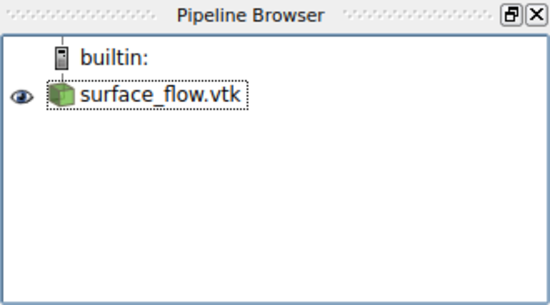
\includegraphics[width=0.4\textwidth]{tut03/surface_flow.pdf}
    \caption{Loading \textit{surface\_flow}.vtk file in the \textbf{Pipeline Browser}.}
    \label{fig:load}
\end{figure}
%--------------------------------------------------------------
\subsection{Visualize Mesh Domain}
In order to view mesh, according to Fig.\ref{fig:wireframe}, select \textit{Solid Color} with \textit{Wireframe} in the toolbar. As you can see from Fig.\ref{fig:mesh}, the mesh around the ONERA M6 wing is unstructured, and the grids are clustered around the tip, leading and trailing edges of the wing. The reason for this clustering is that the changes in flow variables are high at these regions and the mesh should be fine enough at vicinity of these regions in order to solve flow accurately.
\begin{figure}[htbp]
    \centering
    \includegraphics[width=0.6\textwidth]{tut03/wireframe.pdf}
    \caption{How to display mesh in computational domain.}
    \label{fig:wireframe}
\end{figure}
\begin{figure}[htbp]
    \centering
    \includegraphics[width=.75\textwidth]{tut03/mesh2.pdf}
    \caption{Unstructured mesh around ONERA M6 wing.}
    \label{fig:mesh}
\end{figure}
%--------------------------------------------------------------
\subsection{Visualize Pressure Coefficient Contour and Much Number Contour}
To display the pressure contour, click on the \textit{surface\_flow}.vtk in the \textbf{Pipeline Browser}, and then click on the \textbf{Display} in \textbf{Properties} tab. Next, under \textbf{Coloring}, select \textit{Pressure\_Coefficient} from drop-down menu (Fig.\ref{fig:pressure_coeff_1}).
\begin{figure}[htbp]
    \centering
    \includegraphics[width=0.4\textwidth]{tut03/coloring.pdf}
    \caption{Display contour by selecting variable.}
    \label{fig:pressure_coeff_1}
\end{figure}
Eventually, the pressure coefficient contour should be similar to Fig.\ref{fig:plot_pressure_coeff}
\begin{figure}[htbp]
    \centering
    \includegraphics[width=0.65\textwidth]{tut03/cont1_pressure_coefficient.pdf}
    \caption{Pressure coefficient contour for ONERA M6 wing.}
    \label{fig:plot_pressure_coeff}
\end{figure}

In order to add contour lines to the plot, click again on the \textit{surface\_flow}.vtk in the \textbf{Pipeline Browser}, and then click on the \textbf{Contour} icon (Fig.\ref{fig:contour_icon}) in toolbar.
\begin{figure}[htbp]
    \centering
    \includegraphics[width=0.5\textwidth]{tut03/contourlineicon.pdf}
    \caption{\textbf{Contour} icon in toolbar.}
    \label{fig:contour_icon}
\end{figure}
Eventually, \textit{Contour1} appears under \textit{flow}.vtk file in the \textbf{Pipeline Browser} (Fig.\ref{fig:contour1}). Then, click on \textbf{Apply} to proceed next step.
\begin{figure}[htbp]
    \centering
    \includegraphics[width=0.4\textwidth]{tut03/contour1.pdf}
    \caption{Adding \textit{Contour1} in \textbf{Pipeline Browser}.}
    \label{fig:contour1}
\end{figure}
According to Fig.\ref{fig:contourby a}, go to the \textbf{Properties}, and choose \textit{Pressure\_Coefficient} from \textbf{Contour By} drop-down menu. Then, click on the \textbf{Add Range} icon to customize the range of pressure contour. As seen from Fig.\ref{fig:contourby b},  max/min (i.e. \textbf{From}/\textbf{To}) range of contour lines, as well as the number steps required to divide this range into the equal portions exist. So, set \textbf{Step} to 20, and click on \textbf{OK}. At the end, click on \textbf{Apply} to illustrate contour lines in display window.
\begin{figure}[htbp]
    \centering
     \begin{subfigure}[b]{.4\textwidth}
         \centering
         \includegraphics[width=1.0\textwidth]{tut03/pressure_coeff_addrange1.pdf}
         \caption{Define new range}
         \label{fig:contourby a}
     \end{subfigure}
     \hfill
     \begin{subfigure}[b]{.4\textwidth}
         \centering
         \includegraphics[width=1.0\textwidth]{tut03/pressure_coeff_addrange2.pdf}
         \caption{Add range}
         \label{fig:contourby b}
     \end{subfigure}     
    \caption{How to define a new range for the contour lines.}
    \label{fig:contourby}
\end{figure}
Next, as it is shown in Fig.\ref{fig:colorby2}, click on the \textbf{Display} under \textbf{Properties} tab. In \textbf{Coloring} section, select \textbf{Solid Color} form drop-down menu, and choose black color from \textbf{Edit}.
\begin{figure}[htbp]
    \centering
    \includegraphics[width=0.4\textwidth]{tut03/coloring2.pdf}
    \caption{Changing contour lines color in \textbf{Coloring} section.}
    \label{fig:colorby2}
\end{figure}
Eventually, the pressure contour with black contour lines should be similar to Fig.\ref{fig:pressure_contour_lines}.
\begin{figure}[htbp]
    \centering
    \includegraphics[width=.65\textwidth]{tut03/cont2_pressure_coefficient.pdf}
    \caption{Pressure coefficient contour superimposed by contour lines for ONERA M6 wing.}
    \label{fig:pressure_contour_lines}
\end{figure}

To display the Mach number contour, similar to Fig.\ref{fig:pressure_coeff_1}, click on the \textit{surface\_flow}.vtk in the \textbf{Pipeline Browser}, and under \textbf{Coloring} from \textbf{Display}, select \textit{Mach} from drop-down menu. In the next step, click on "\textit{Contour1}" in the \textbf{Pipeline Browser}. As it is shown in Fig.\ref{fig:contourby2 a}, under \textbf{Properties}, select \textit{Mach} from \textbf{Contour By} drop-down menu. Next, click on \textbf{Remove All} icon to remove previous value range belonged to pressure coefficient. Similar to Fig.\ref{fig:contourby2 b}, click on \textbf{Add Range} icon and set \textbf{Steps} to 20. Next, click on \textbf{OK}, and then, \textbf{Apply} to show plot.
\begin{figure}[htbp]
    \centering
     \begin{subfigure}[b]{.4\textwidth}
         \centering
         \includegraphics[width=1.0\textwidth]{tut03/del_add_range_mach.pdf}
         \caption{Define new range}
         \label{fig:contourby2 a}
     \end{subfigure}
     \hfill
     \begin{subfigure}[b]{.4\textwidth}
         \centering
         \includegraphics[width=1.0\textwidth]{tut03/AddRangemach.pdf}
         \caption{Add range}
         \label{fig:contourby2 b}
     \end{subfigure}     
    \caption{How to define a new range for the contour lines.}
    \label{fig:contourby2}
\end{figure}
Now the Mach number contour of the wing surface should be similar to Fig.\ref{fig:mach_contour}.
\begin{figure}[htbp]
    \centering
    \includegraphics[width=0.5\textwidth]{tut03/machcontour1.pdf}
    \caption{Mach number contour with superimposed by lines.}
    \label{fig:mach_contour}
\end{figure}
%--------------------------------------------------------------
\subsection{Comparison of Convergence Rate}
Launch Microsoft Excel or any other plotting software. For Microsoft Excel, open the file \textit{history}.vtk from the tutorial folder. Then, you are asked to choose the file type that best describes your data. You should select \textbf{Delimiters}, and in the next step, Under the \textbf{Delimiters}, select only the check boxes for \textit{Tab}, \textit{Semicolon}, and \textit{Comma} (Fig.\ref{Fig11}).
\begin{figure}[htbp]
    \centering
    \includegraphics[width=0.5\textwidth]{tut03/16.png}
    \caption{Import .vtk file in Microsoft Excel.}
    \label{Fig11}
\end{figure}
As shown in Fig.\ref{Fig12}, the first column shows the iteration number. The lift coefficient ($C_L$) and the drag coefficient ($C_D$) are displayed in the second and third column, respectively. Additionally, the residuals can also be examined to check convergence (Column \textit{L} to Column \textit{P} in Fig.\ref{Fig13}).
\begin{figure}[htbp]
    \centering
    \includegraphics[width=0.5\textwidth]{tut03/17.png}
    \caption{Columns in \textit{history}.vtk}
    \label{Fig12}
\end{figure}
\begin{figure}[htbp]
    \centering
    \includegraphics[width=0.75\textwidth]{tut03/18.png}
    \caption{Residuals in \textit{history}.vtk}
    \label{Fig13}
\end{figure}
Now we plot the lift coefficient, drag coefficient, and density residual against the number of iterations to see how many iterations it takes to converge to a steady solution. Fig.\ref{Fig14} and Fig.\ref{Fig15} shows the plots for aerodynamic loads and residual versus the number of iterations, respectively, for the case of \texttt{MGLEVEL=0} on tetrahedral mesh.
\begin{figure}[htbp]
    \centering
    \includegraphics[width=0.75\textwidth]{tut03/22.png}
    \caption{Lift and Drag coefficients versus the number of iterations.}
    \label{Fig14}
\end{figure}
\begin{figure}[htbp]
    \centering
    \includegraphics[width=0.75\textwidth]{tut03/21.png}
    \caption{Density residual versus the number of iterations.}
    \label{Fig15}
\end{figure}
%++++++++++++++++++++++++++++++++++++++++++++++++++++++++++++++
\section{Questions}
1. Run the simulation without multi-grid scheme (\texttt{MGLEVEL=0}).
\begin{enumerate}[label=(\alph*)]
    \item Follow the procedure in the guideline document to run the simulation and record the number of iterations and wall-clock time for the simulation to complete.
    \item Record the lift and drag coefficients.
    \item Plot the surface pressure coefficient with coloured contours and contour lines.
    \item Plot the surface Mach number with coloured contours and contour lines.
    \item Plot the value of Cd, Cl and the density residual vs. the number of iterations.
\end{enumerate}\\
2. Modify the configuration file in the multi-grid folder (\texttt{MGLEVEL= 3, MGCYCLE= W\_CYCLE}) and repeat Q.1 using multi-grid scheme.\\
3. Compare the results in part (a)-(e) of Q.1 and Q.2. In what way is the use of multi-grid advantageous for this test case?\\
%++++++++++++++++++++++++++++++++++++++++++++++++++++++++++++++
\chapter{Laminar Flat Plate}

\chapter{Laminar Cylinder}

\chapter{Turbulent ONERA M6}
